\documentclass[10pt]{beamer}

%% metropolis
\usetheme[progressbar=frametitle]{metropolis}
\makeatletter
    \definecolor{uosblue}{RGB}{10, 77, 155}
    \definecolor{pytorchorange}{RGB}{238, 76, 44}
    \setbeamercolor{background canvas}{bg=white}
    %\setbeamercolor{normal text}{fg=lightbeige}
    \setbeamercolor{frametitle}{bg=uosblue}
    \setbeamercolor{progress bar}{fg=black, bg=lightgray}
    \setbeamercolor{section in head}{bg=white}
    \setlength{\metropolis@titleseparator@linewidth}{2pt}
    \setlength{\metropolis@progressonsectionpage@linewidth}{2pt}
    \setlength{\metropolis@progressinheadfoot@linewidth}{2pt}
    %% https://github.com/eddelbuettel/pkg-latex-metropolis/blob/master/usr/share/texmf/tex/latex/metropolis/beamerfontthememetropolis.sty
    \setbeamerfont{title}{size=\large}
    \setbeamerfont{author}{size=\footnotesize}
    \setbeamertemplate{caption}{\insertcaption} 
\makeatother

%% usepackage
\usepackage{appendixnumberbeamer}
\usepackage{amsmath}
\usepackage{graphicx}
%\usepackage{enumitem}
\usepackage{hyperref}
\usepackage{minted}
\usepackage{emoji}



%% more setup
\hypersetup{colorlinks,linkcolor=uosblue,urlcolor=uosblue}
\setemojifont{TwemojiMozilla}


%%%%%%%%%%%%%%%%%%%%%%%%%%%%%%%%%%%%%%%%%%%%%%%%%%%%%%%%%%%%%%%%%%
\newcommand{\pytorch}{{\color{pytorchorange} PyTorch}}
\newcommand{\disclaimer}[1]{{\color{red} \textbf{\emph{{\scriptsize DISCLAIMER}}}}\,{{\scriptsize \textit{#1}}}}
\newcommand{\RunII}{Run{\uppercase\expandafter\romannumeral 2}}
\newcommand{\PhaseII}{Phase{\uppercase\expandafter\romannumeral 2}}

\newcommand{\TODO}{{\color{red} \textbf{TODO}}}


%%%%%%%%%%%%%%%%%%%%%%%%%%%%%%%%%%%%%%%%%%%%%%%%%%%%%%%%%%%%%%%%%%
\title{Muon Segment Reconstruction with ML}
%\subtitle{Deep Learning-based Background Hit Removal}

\author{
    Seungjin Yang \\
    University of Seoul % positioning problem
}

%
%\institute[VFU]{University of Seoul}

\date{
    January 14, 2022 \\
    LHC KCMS Annual Workshop 
}


% logo
\titlegraphic{
   \hfill
   
\includegraphics[width=1.6cm]{figures/misc/uni-logo.png}
   
\includegraphics[width=1.1cm]{figures/misc/CMSlogo_outline_black_label.pdf}
}

\begin{document}

%%%%%%%%%%%%%%%%%%%%%%%%%%%%%%%%%%%%%%%%%%%%%%%%%%%%%%%%%%%%%%%%%%
\begin{frame}[noframenumbering,plain]
    \maketitle
\end{frame}


\begin{frame}[fragile]{Introduction}
\begin{itemize}
    \item[$\blacksquare$] The GE0 (ME0) module is six layers of triple-GEM.
    \begin{itemize}
        \item Extend the acceptance of the CMS muon system to $\vert\eta\vert=2.8$.
        \item Keep or improve the muon trigger efficiency in the harsh environment of \PhaseII.
        \item Also, improve the offline muon reconstruction.
    \end{itemize}
    \item[$\blacksquare$] The current offline segment building algorithm for GE0 is \href{https://github.com/cms-sw/cmssw/blob/master/RecoLocalMuon/GEMSegment/plugins/GE0SegAlgoRU.h}{Road Usage (RU)}, which is an iterative method \href{https://www.epj-conferences.org/articles/epjconf/pdf/2016/03/epjconf_mmcp2016_02023.pdf}{originally developed for the CSC}.% \TODO
    \item[$\blacksquare$] Use Deep Learning (DL) as the background hit removal method and keep Road Usage for the muon segment reconstruction.
\end{itemize}

\begin{figure}
    \centering
    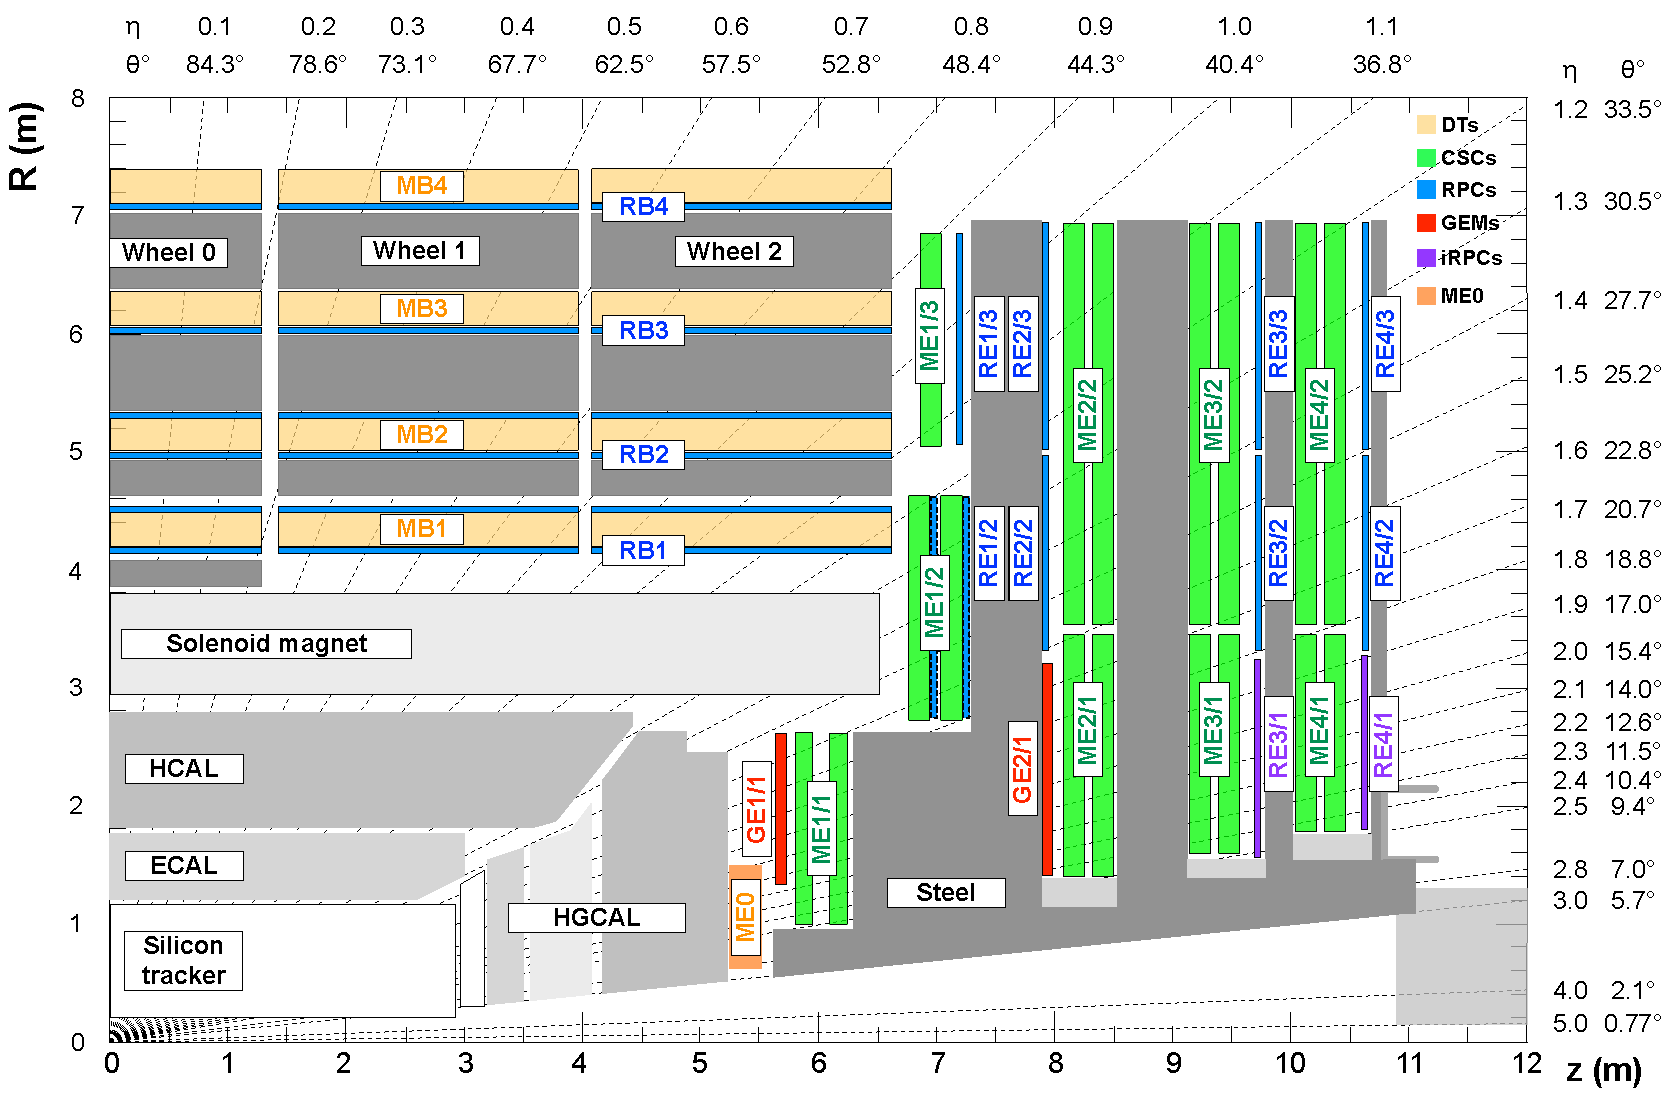
\includegraphics[width=0.32\textwidth]{figures/detector/detectorplacement1.pdf}
    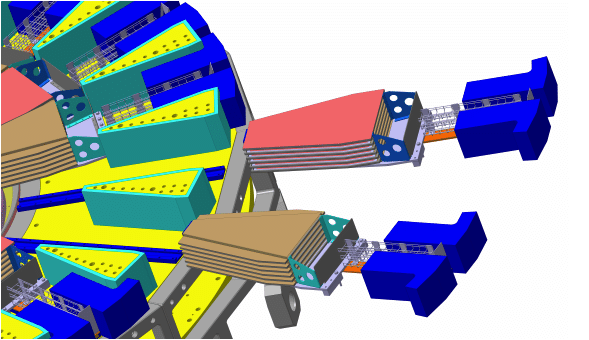
\includegraphics[width=0.32\textwidth]{figures/detector/3D-drawing-of-the-insertion-of-two-adjacent-stacks-of-six-ME0-modules-into-the-end-cap.ppm.png}
    \href{https://www.epj-conferences.org/articles/epjconf/pdf/2019/19/epjconf_chep2018_02014.pdf}{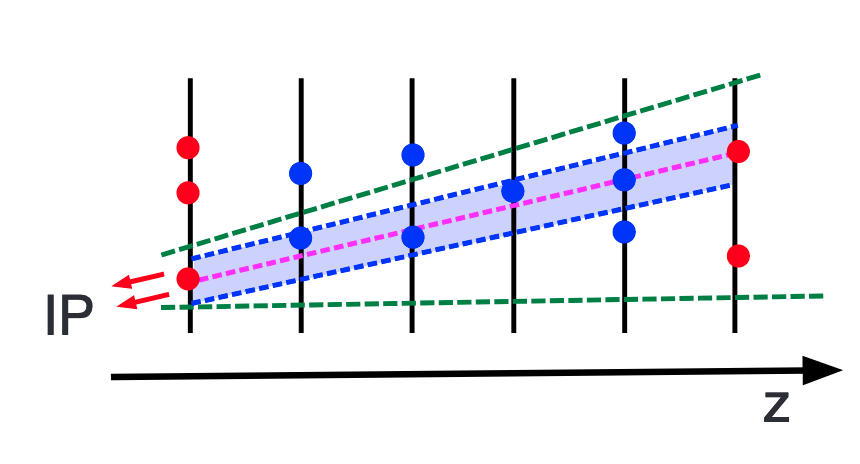
\includegraphics[width=0.32\textwidth]{figures/RU/Schematic-illustration.png}}
    %\caption{Caption}
    %\label{fig:my_label}
\end{figure}

\end{frame}

%%%%%%%%%%%%%%%%%%%%%%%%%%%%%%%%%%%%%%%%%%%%%%%%%%%%%%%%%%%%%%%%%%
\begin{frame}[fragile]{Segment Reconstruction with Background Hit Removal}
\begin{figure}
    \centering
    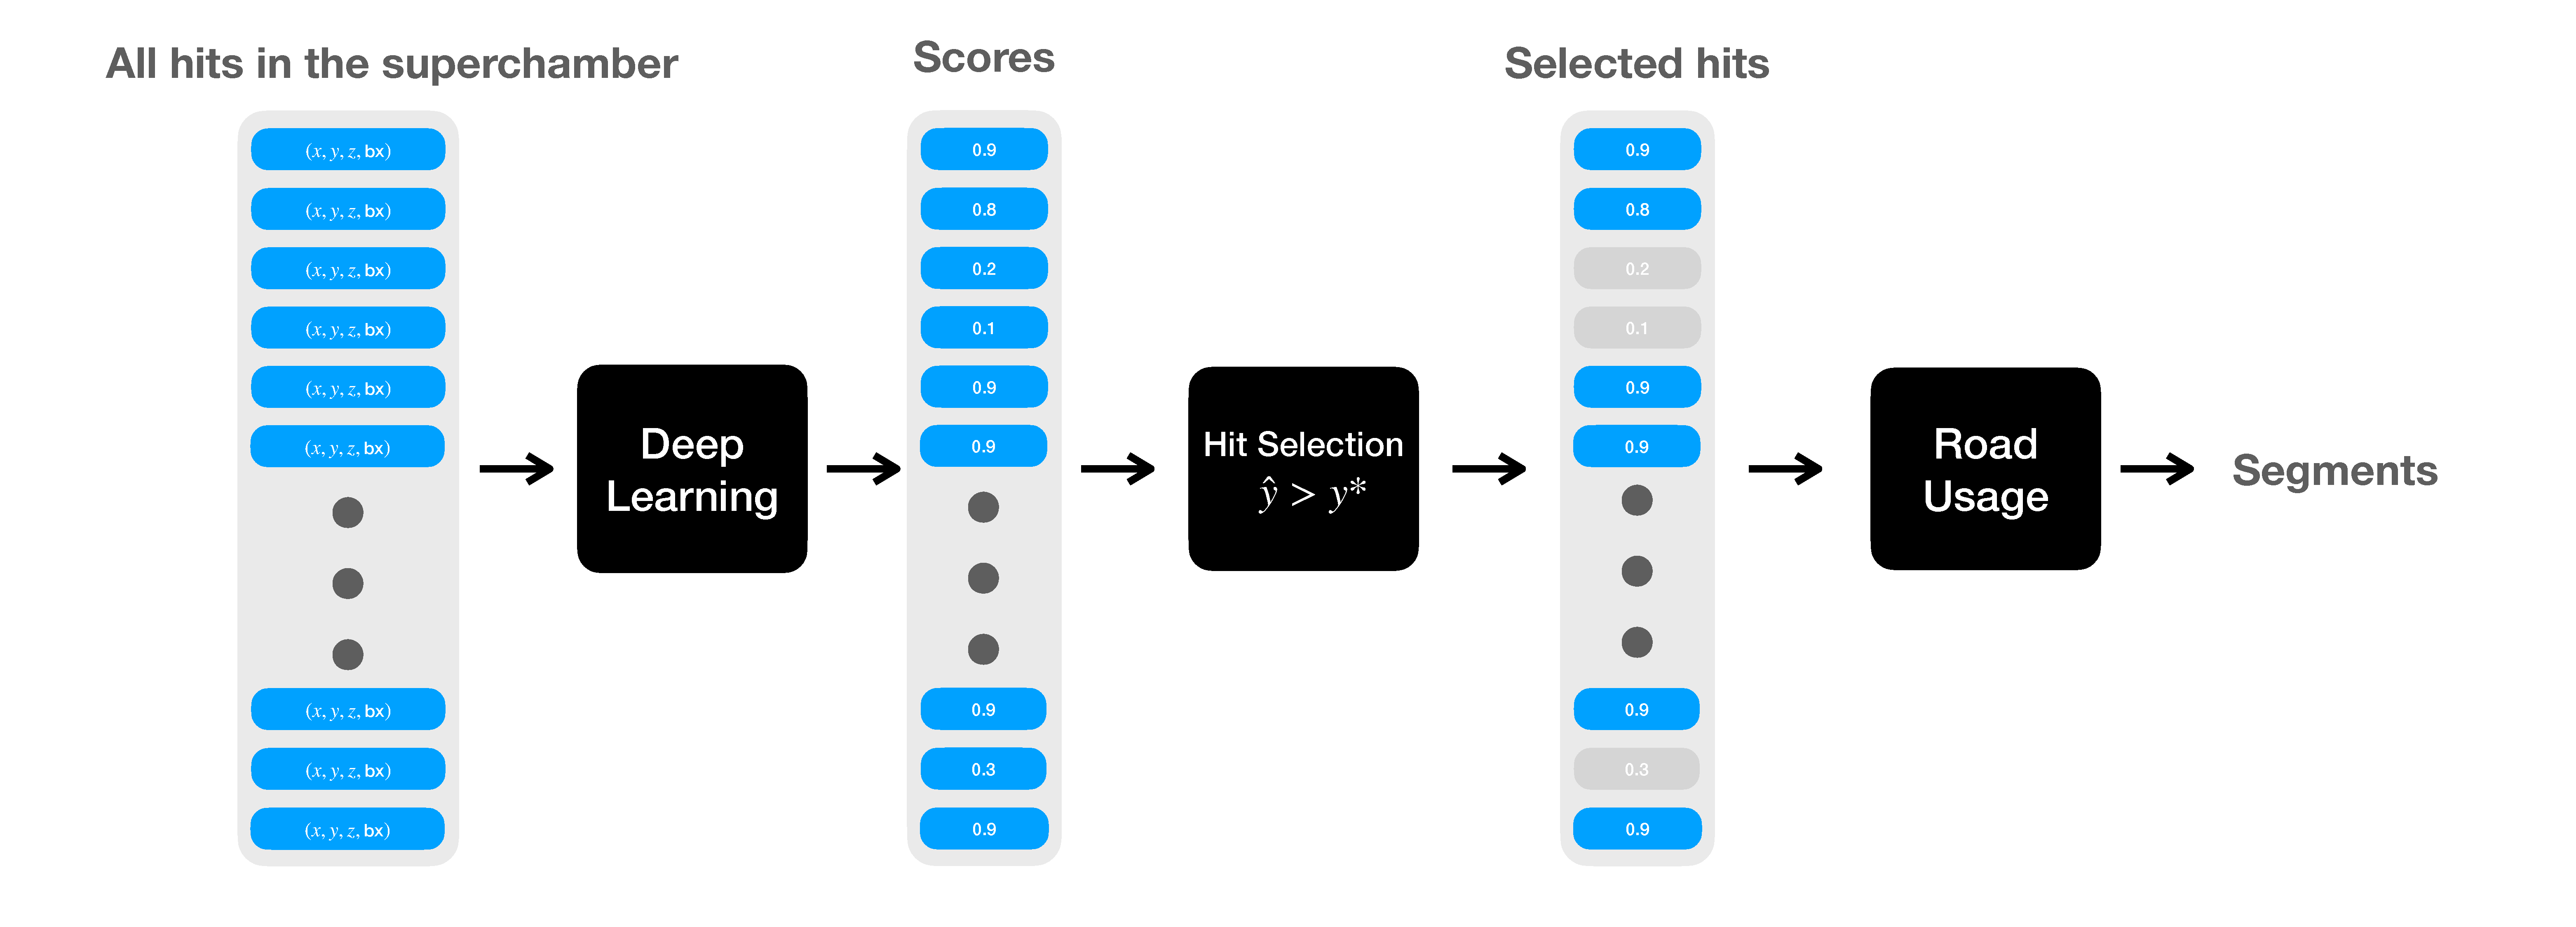
\includegraphics[width=\textwidth]{figures/model/workflow.pdf}
    %\caption{Caption}
    %\label{fig:my_label}
\end{figure}
\end{frame}


%%%%%%%%%%%%%%%%%%%%%%%%%%%%%%%%%%%%%%%%%%%%%%%%%%%%%%%%%%%%%%%%%%

\begin{frame}[fragile]{Background Hit Removal via Deep Learning: The Task}
\begin{itemize}
    \item \textbf{Background hit removal = Hit-wise binary classification}
    \item The model $f$ takes all hits $\{\mathbf{x}^{(1)}, \ldots, \mathbf{x}^{(N)}\}$ in the GE0 superchamber and then produces a score $\hat{y}^{(n)}$ for each hit.
    \begin{equation*}
        f: 
        \begin{bmatrix}
            \mathbf{x}^{(1)} \\
            \mathbf{x}^{(2)} \\
            \vdots \\
        \mathbf{x}^{(N)}
            \end{bmatrix}
        \rightarrow
        \begin{bmatrix}
            \hat{y}^{(1)} \\
            \hat{y}^{(2)} \\
            \vdots \\
            \hat{y}^{(N)} \\
        \end{bmatrix}
    \end{equation*}
    \item The features of the hit: the position in the superchamber frame and the bunch crossing.
    \begin{equation*}
        \text{Hit} = \mathbf{x} = \left( x, y, z, \text{bx} \right)
    \end{equation*}
    \item If the hit is the muon hit, the label $y$ is 1. If not , the label is 0.
\end{itemize}


\end{frame}


%%%%%%%%%%%%%%%%%%%%%%%%%%%%%%%%%%%%%%%%%%%%%%%%%%%%%%%%%%%%%%%%%%
\begin{frame}[fragile]{Background Hit Removal via Deep Learning: The Experience}

\begin{itemize}
    \item[$\blacksquare$] Objective function: \href{https://pytorch.org/docs/1.10.0/generated/torch.nn.BCEWithLogitsLoss.html}{the weighted binary cross entropy}
    \begin{equation*}
        J\left(\textbf{\theta}\right)= \frac{1}{N} \sum_{n=1}^{N} -\left(w_{+} y^{(n)}\cdot \log{\hat{y}^{(n)}} + \left( 1-y^{(n)} \right) \cdot \log{ \left(1 - \hat{y}^{(n)} \right) }\right)
    \end{equation*}
    \begin{itemize}
        \item $N$ is the number of hits in the superchamber
        \item $w_{+}=\frac{\text{the number of background hits}}{\text{the number of muon hits}}$.
    \end{itemize}
    \item[$\blacksquare$] Optimization algorithm: \href{https://arxiv.org/abs/1412.6980}{Adam} with L2 penalty.
    \item[$\blacksquare$] \href{https://github.com/pytorch/pytorch}{\pytorch}\ v.1.10.0
    \item [$\blacksquare$] No hyperparameter optimization is performed.
\end{itemize}

\end{frame}


%%%%%%%%%%%%%%%%%%%%%%%%%%%%%%%%%%%%%%%%%%%%%%%%%%%%%%%%%%%%%%%%%%
\begin{frame}[fragile]{Model Architecture}

\begin{columns}
    \begin{column}{0.6\textwidth}
    \begin{itemize}
        \item The model implementation is based on \href{https://arxiv.org/abs/1706.03762}{Transformer}, which is the neural machine translation model and features self-attention.
        \item Self-attention performs a weight sum of the elements (vectors) of the input, where the weight matrix is also computed from the elements.
        \begin{itemize}
            \item Sentence = a set of words
            \item Image = a set of pixels
            \item Superchamber = a set of hits
        \end{itemize}
        \item Self-attention based model can learn the dependency between elements.
    \end{itemize}
    
    \end{column}

\begin{column}{0.38\textwidth}
\begin{figure}
    \centering
    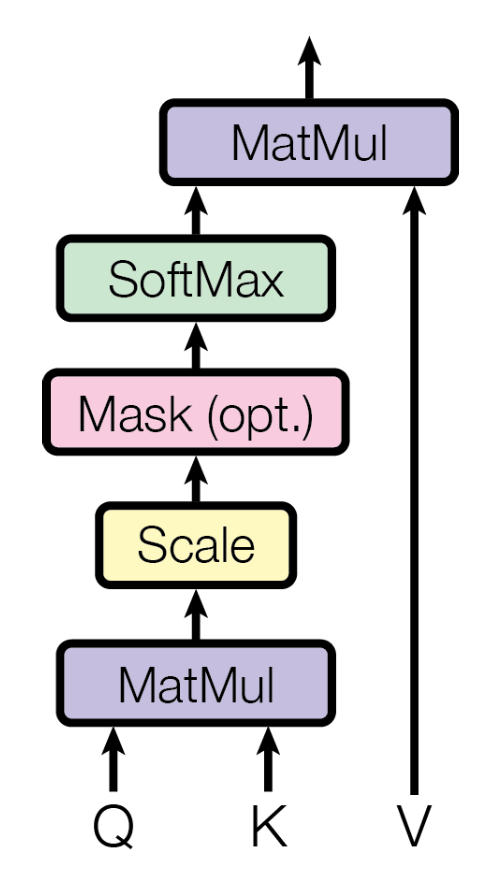
\includegraphics[width=0.6\textwidth]{figures/model/scaled_dot_production_in_paper.png}
    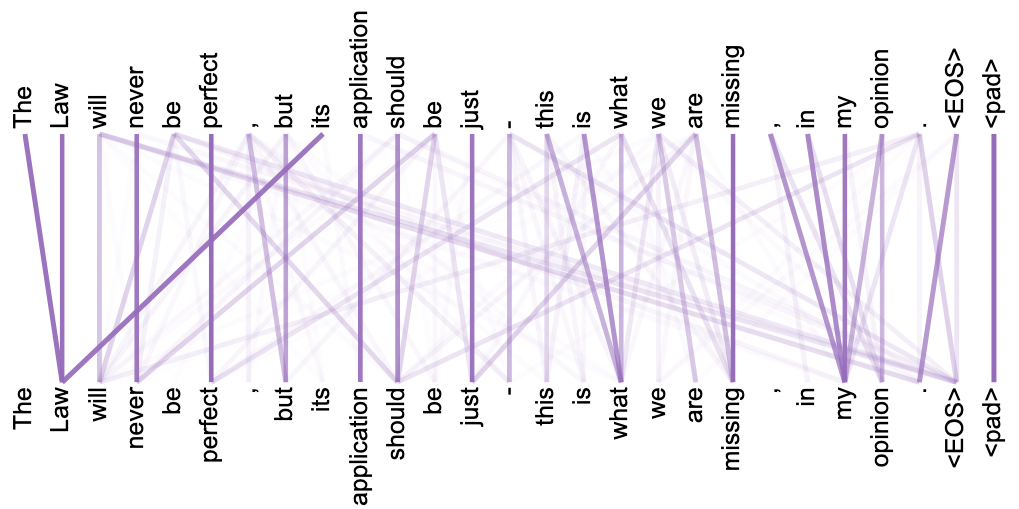
\includegraphics[width=\textwidth]{figures/model/attn-vis.png}
    %\caption{Caption}
    %\label{fig:my_label}
\end{figure}
\end{column}

\end{columns}

\end{frame}


%%%%%%%%%%%%%%%%%%%%%%%%%%%%%%%%%%%%%%%%%%%%%%%%%%%%%%%%%%%%%%%%%%
\begin{frame}[fragile]{Simulation}

$\blacksquare$ Muon gun simulation
\begin{itemize}
    \item 5 GeV < $p_{T}$ < 200 GeV, $1.7 < \vert\eta\vert < 3.2$
    \item The average pile-up of 200.
    \item Geometry: 2026D76 / Era: Phase2C11I13M9 / CMSSW: 12\_0\_0\_pre1
    \item 40k events $\rightarrow$ training : validation : test = 64 : 16 : 20
    \item If the muon leaves 3 or fewer hits in the superchamber, it was considered background.
\end{itemize}


\begin{figure}
    \centering
    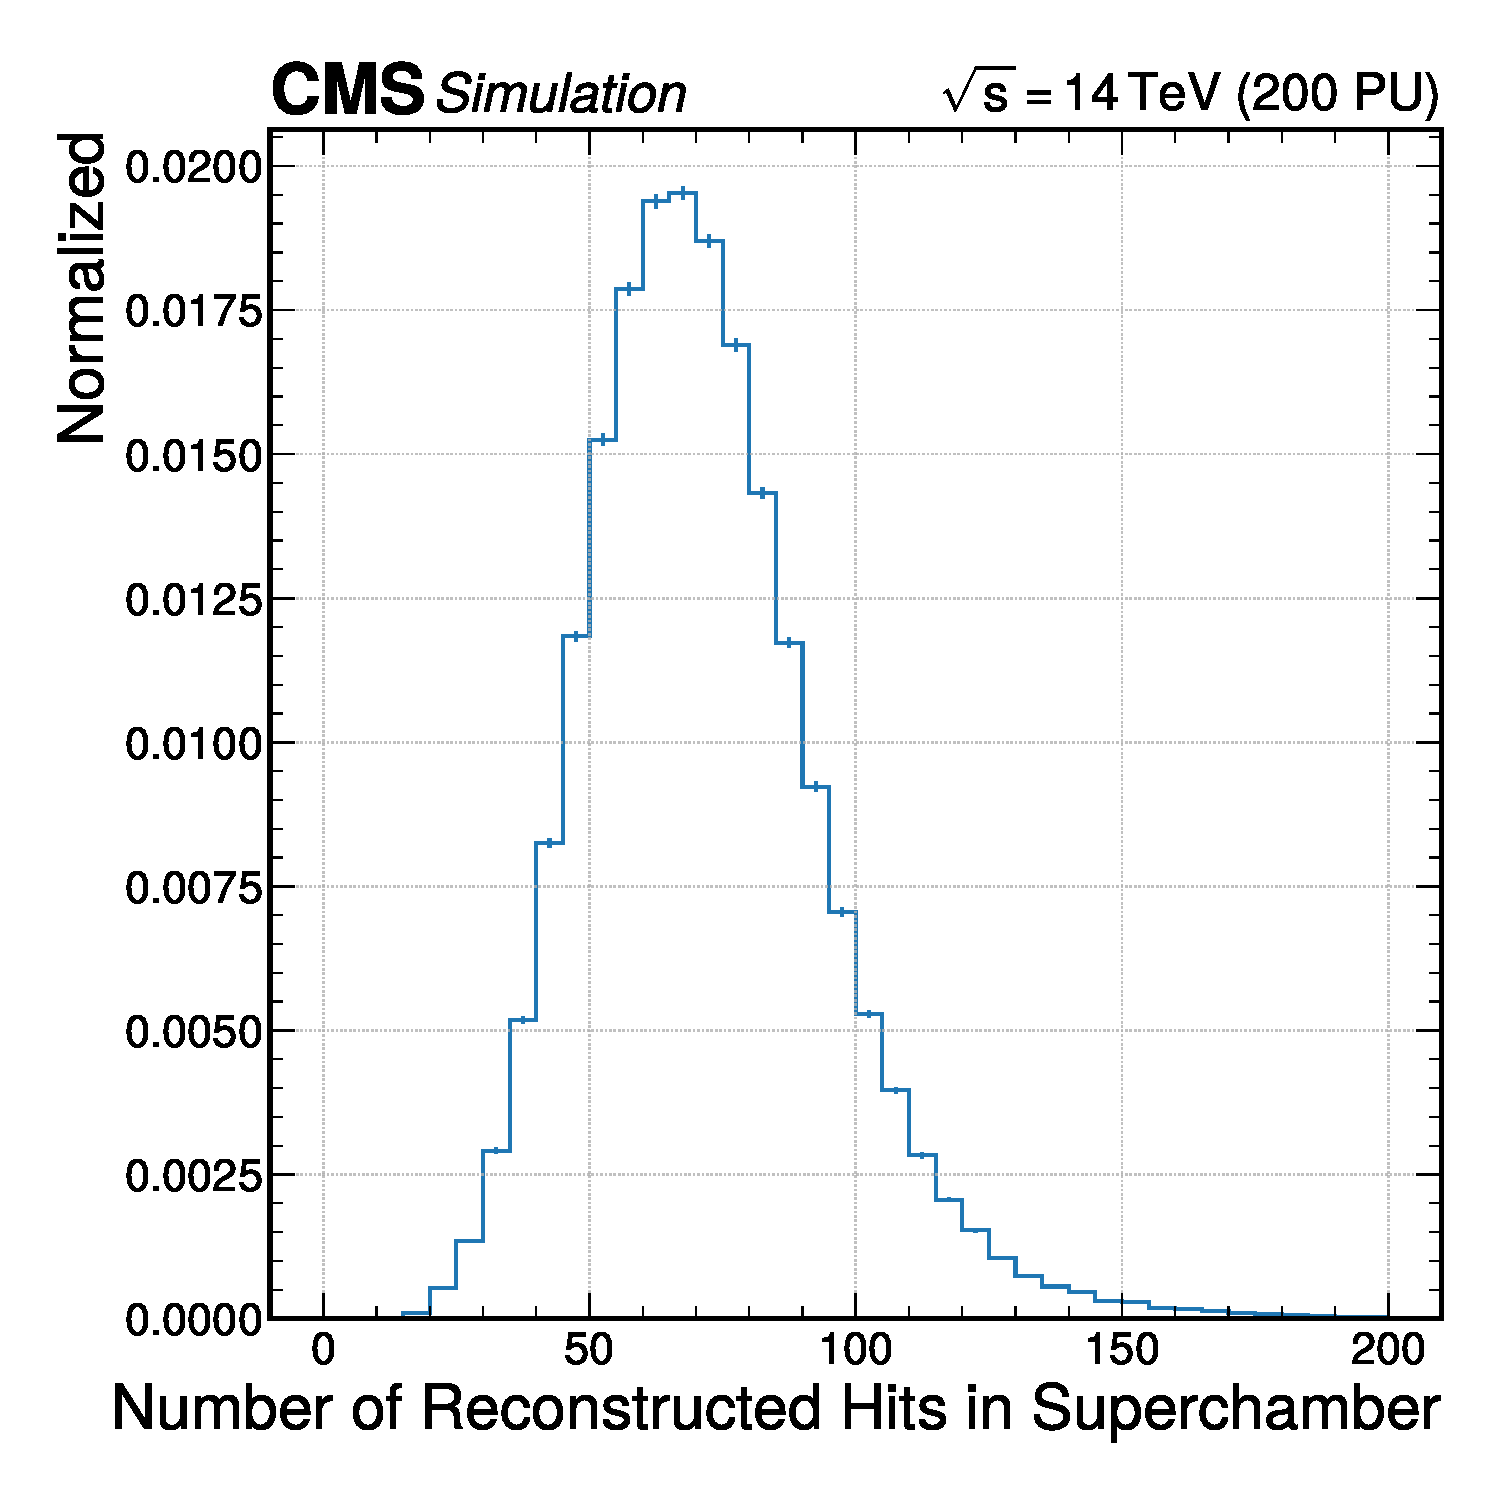
\includegraphics[width=0.32\textwidth]{figures/data/NumHit.pdf}
    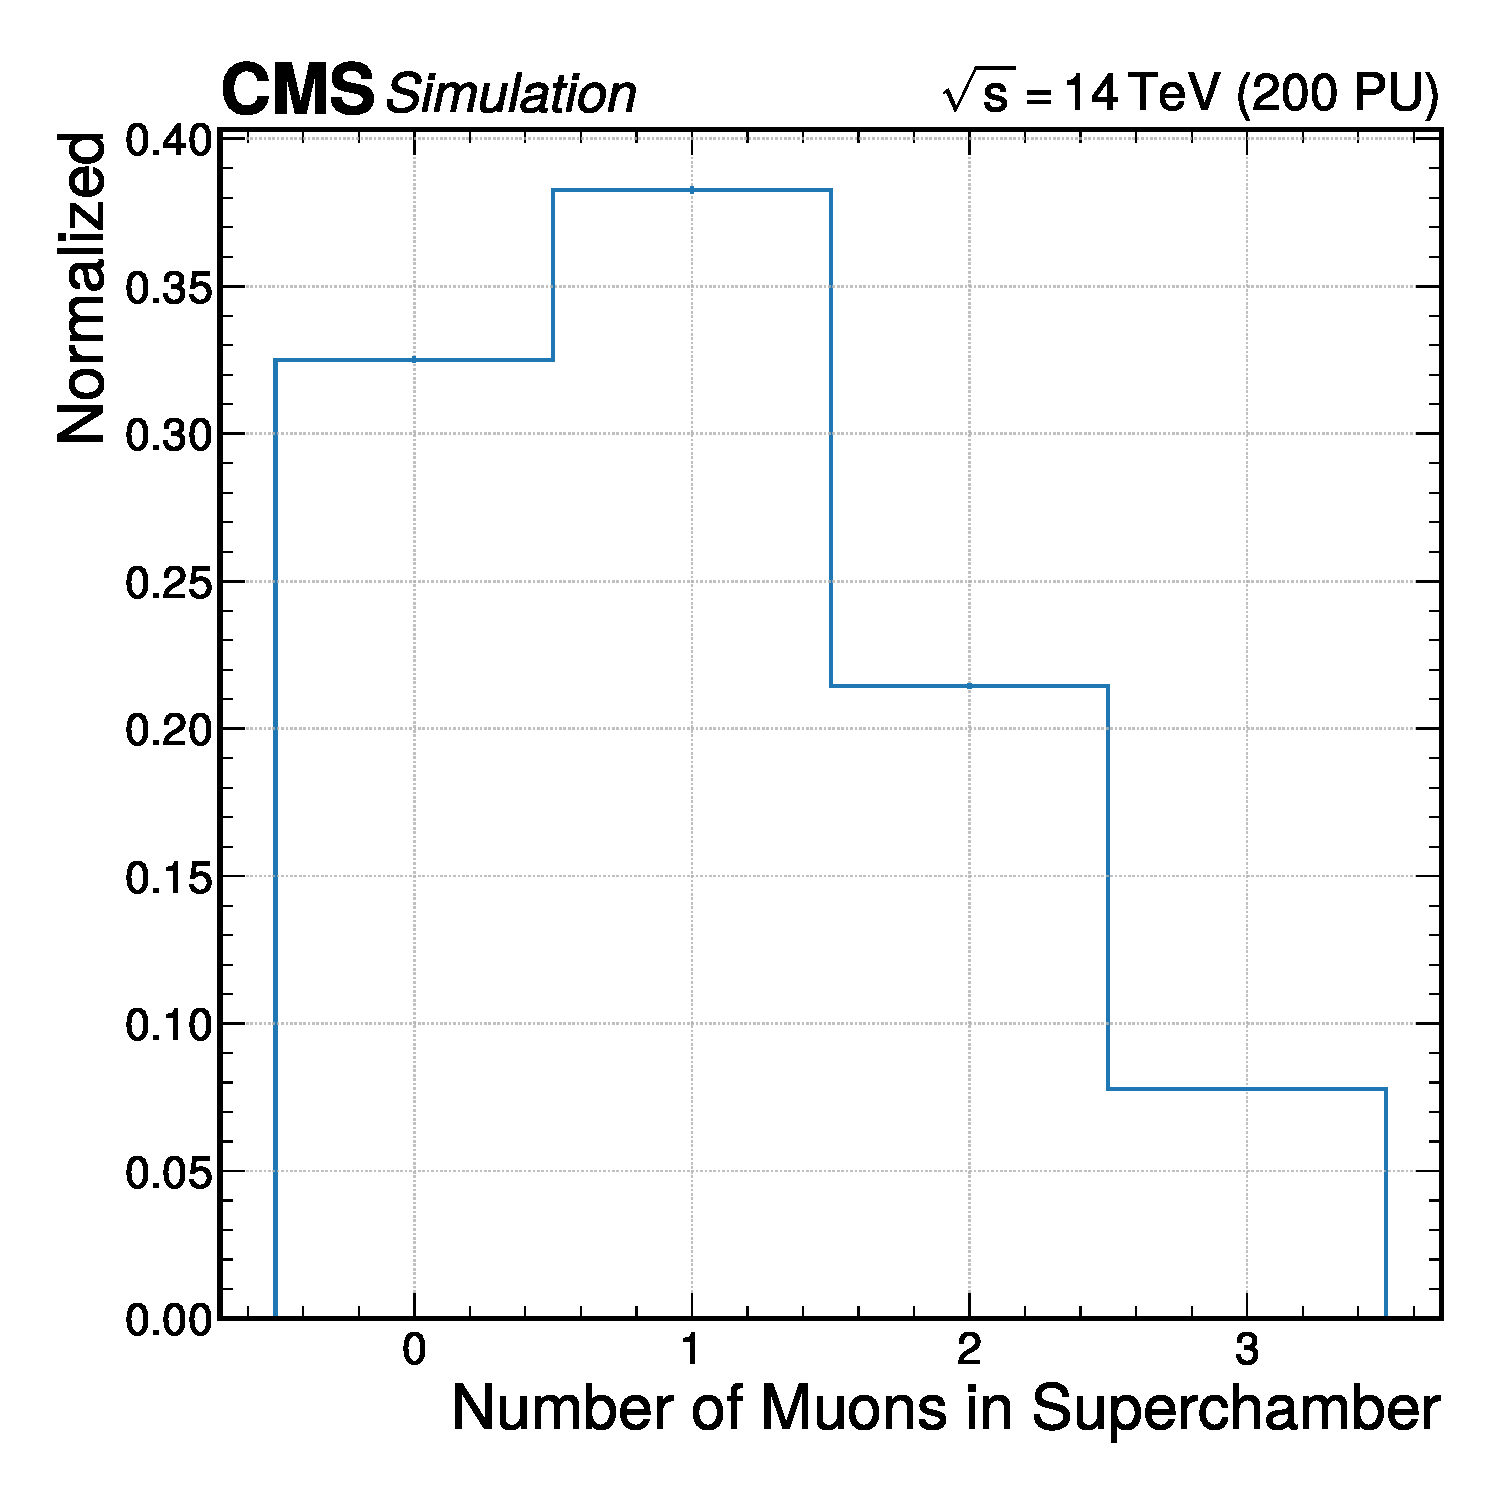
\includegraphics[width=0.32\textwidth]{figures/data/NumMuon.pdf}
    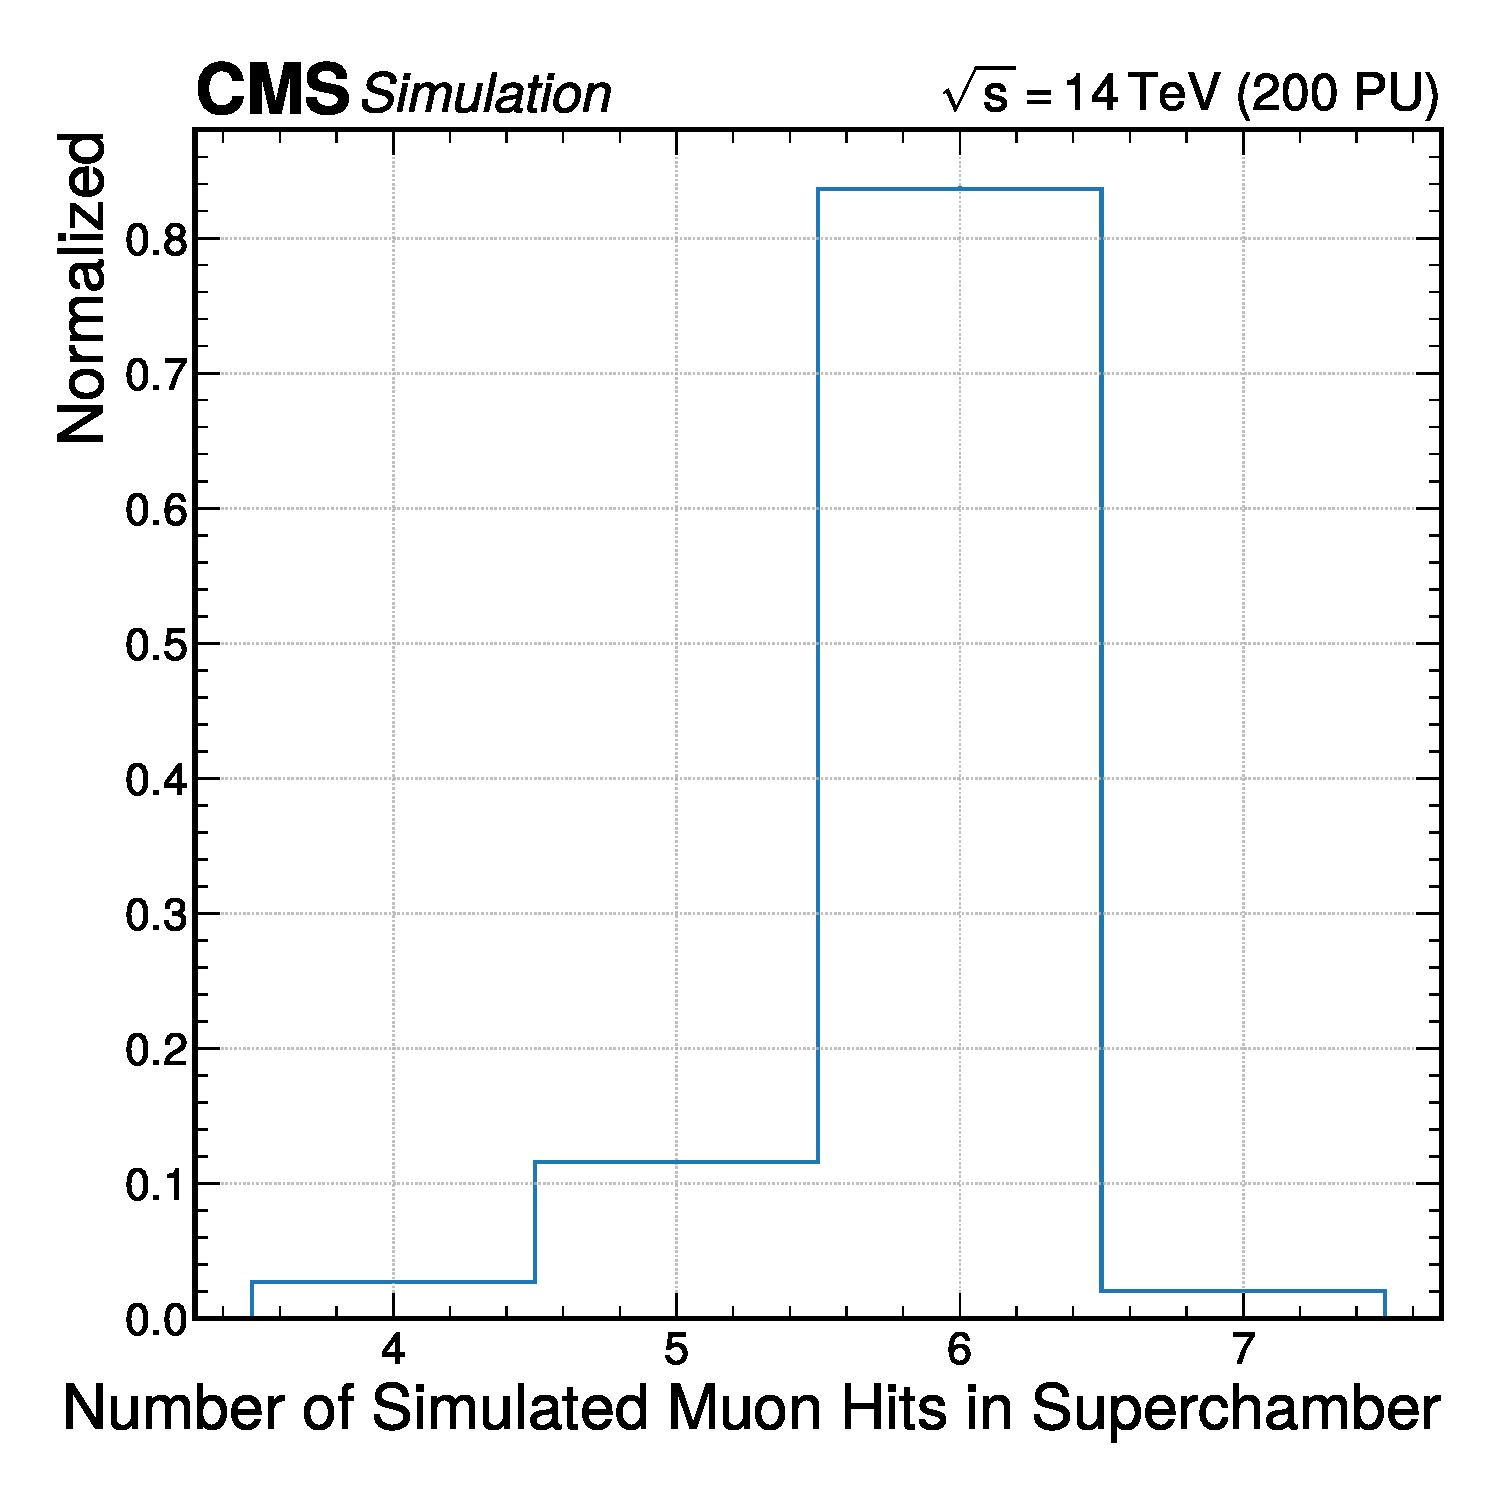
\includegraphics[width=0.32\textwidth]{figures/data/NumMuonHit.pdf}
    %\caption{Caption}
    %\label{fig:my_label}
\end{figure}

\end{frame}


%%%%%%%%%%%%%%%%%%%%%%%%%%%%%%%%%%%%%%%%%%%%%%%%%%%%%%%%%%%%%%%%%%



%%%%%%%%%%%%%%%%%%%%%%%%%%%%%%%%%%%%%%%%%%%%%%%%%%%%%%%%%%%%%%%%%%
\begin{frame}[fragile]{Deep Learning Inference in CMSSW}

\begin{itemize}
    \item[$\blacksquare$] It is required to serialise DL models for deploying it in CMSSW.
    \item[$\blacksquare$] CMSSW has interfaces to the following deep learning platforms.
    \begin{itemize}
        % [\emoji{check-mark}]
        \item \href{https://github.com/microsoft/onnxruntime}{ONNXRuntime} $\rightarrow$ \href{https://github.com/cms-sw/cmssw/tree/master/PhysicsTools/ONNXRuntime}{PhysicsTools/ONNXRuntime}
        \item \href{https://github.com/tensorflow/tensorflow}{TensorFlow} $\rightarrow$ \href{https://github.com/cms-sw/cmssw/tree/master/PhysicsTools/TensorFlow}{PhysicsTools/TensorFlow}
        \item \href{https://github.com/apache/incubator-mxnet}{MXNet} $\rightarrow$ \href{https://github.com/cms-sw/cmssw/tree/master/PhysicsTools/MXNet}{PhysicsTools/MXNet}
    \end{itemize}
    \item[$\blacksquare$] Intermediate representation of \href{https://github.com/pytorch/pytorch}{\pytorch}\ model can be converted to \href{https://github.com/onnx/onnx}{ONNX} format and then CMSSW can deploy it using \href{https://github.com/microsoft/onnxruntime}{ONNXRuntime}.
    \begin{itemize}
        \item \href{https://github.com/onnx/onnx}{ONNX} (Open Neural Network Exchange): An open source format for AI models such as DL or BDT.
        \item \href{https://github.com/microsoft/onnxruntime}{ONNXRuntime}: A cross-platform inference and training ML accelerator.
    \end{itemize}
\end{itemize}
\end{frame}





%%%%%%%%%%%%%%%%%%%%%%%%%%%%%%%%%%%%%%%%%%%%%%%%%%%%%%%%%%%%%%%%%%
\begin{frame}[fragile]{Results}


\begin{figure}
    \centering
    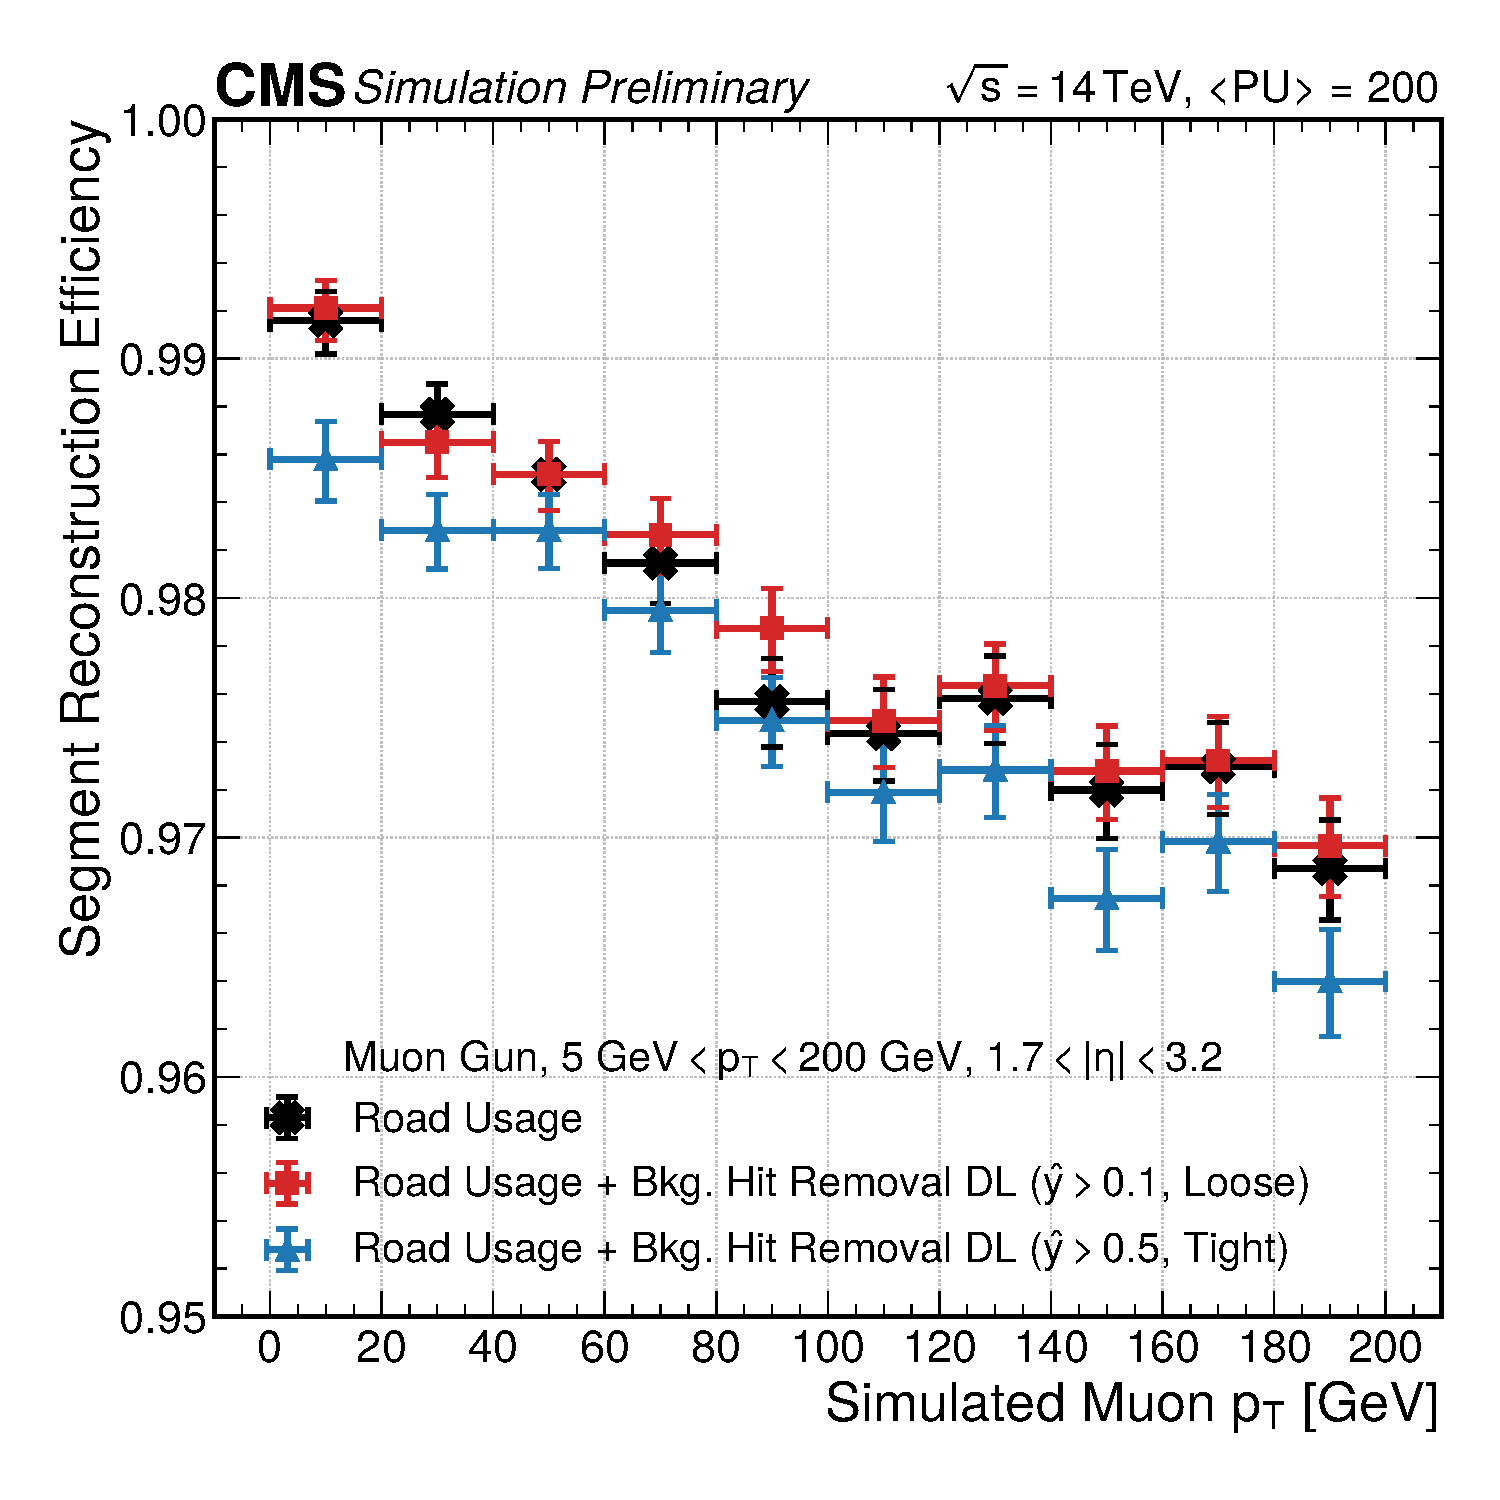
\includegraphics[width=0.32\textwidth]{figures/BkgHitRemoval/eff_muon_pt.pdf}
    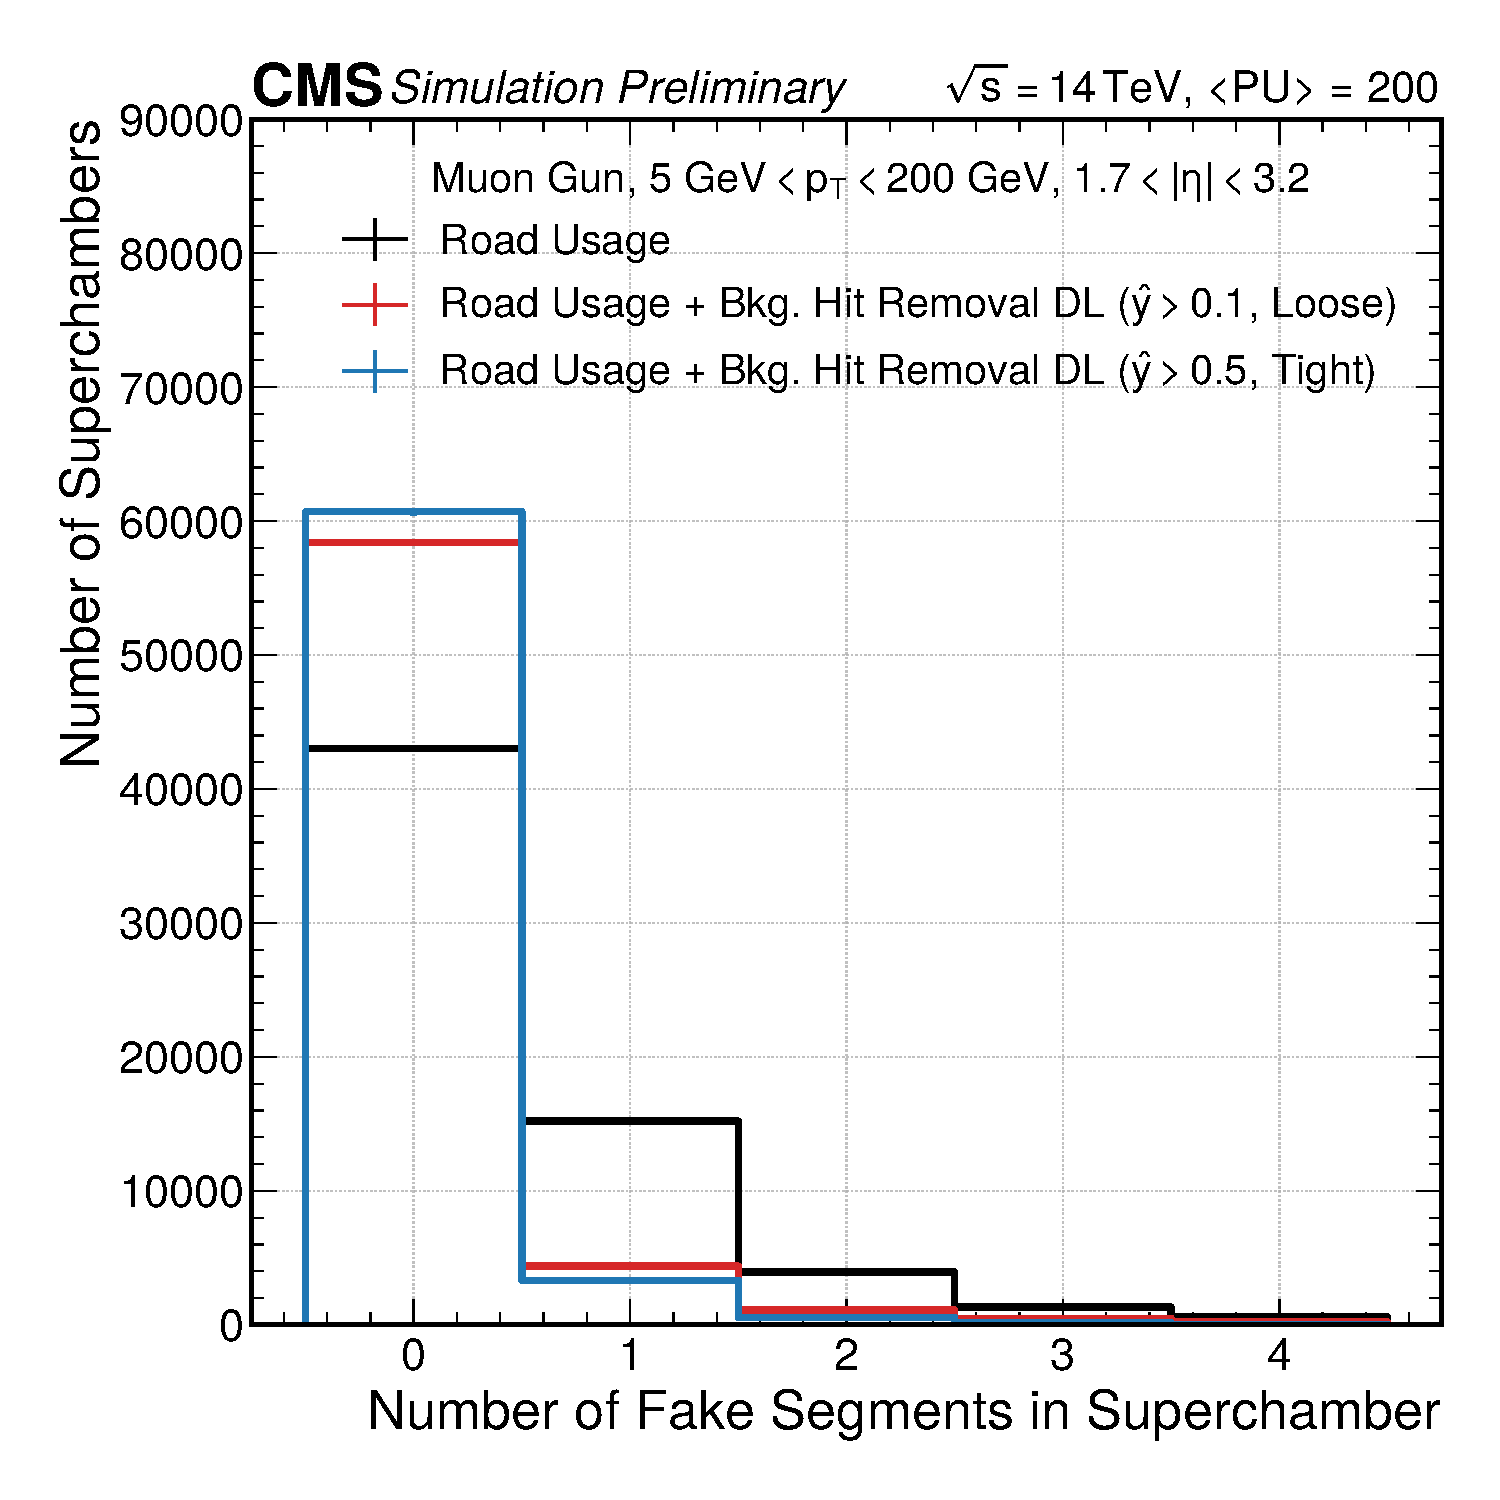
\includegraphics[width=0.32\textwidth]{figures/BkgHitRemoval/num_fake_seg_per_superchamber.pdf}
    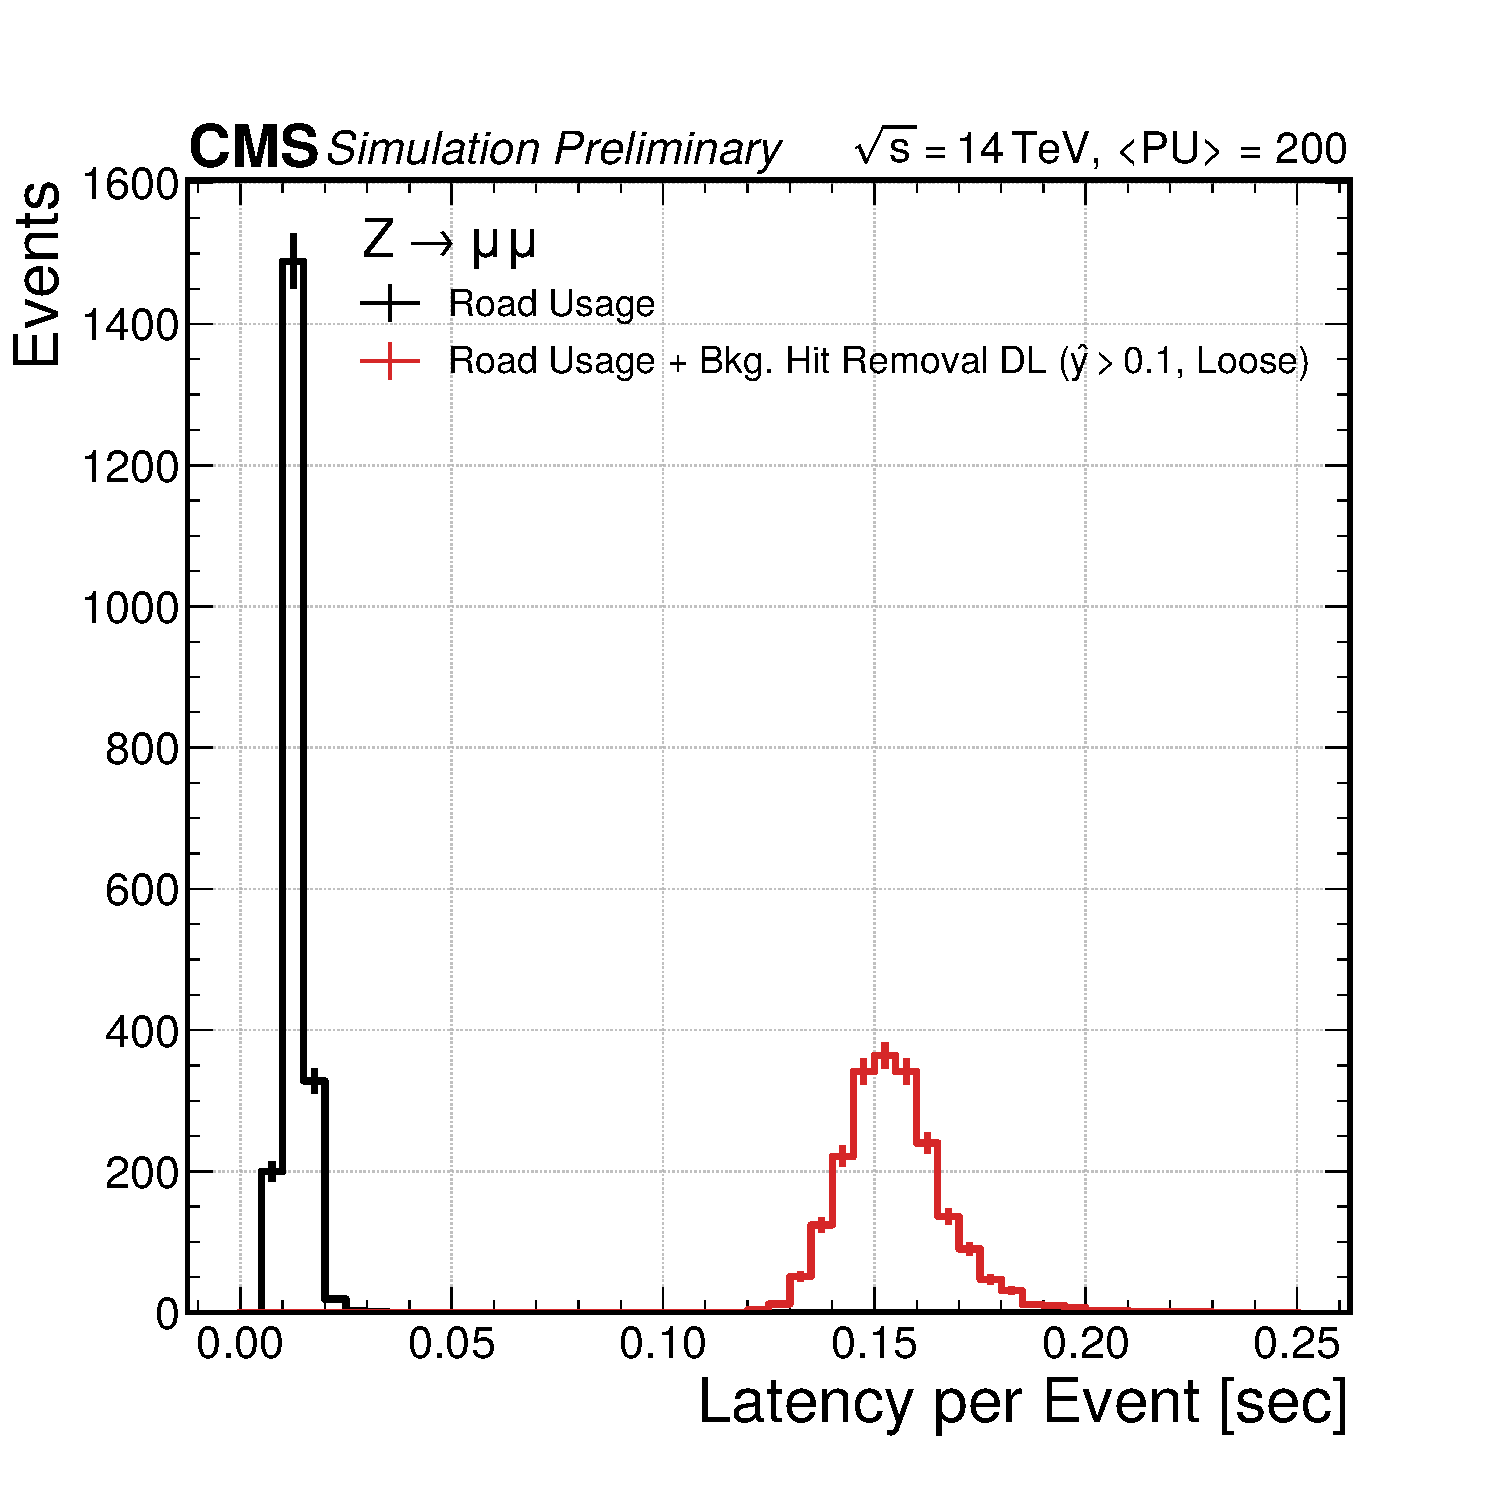
\includegraphics[width=0.32\textwidth]{figures/BkgHitRemoval/latency.pdf}
\end{figure}

\begin{itemize}
    \item[$\blacksquare$] {\small DL-based background hit removal method reduced fake segments while maintaining the efficiency of Road Usage.}
    \item[$\blacksquare$] {\small The size of the resulting DL model is about 0.8 MB.}
    \begin{itemize}
        \item {\footnotesize For comparison, the sizes of DL-based jet taggers are about $0.1 \sim 3$ MB.}
    \end{itemize}
    \item[$\blacksquare$] {\small DL introduced a relatively large overhead. However, it  will need to be re-evaluated during the full reconstruction step. }
    \begin{itemize}
        \item {\footnotesize Latency: \href{https://github.com/cms-sw/cmssw/blob/master/FWCore/Services/plugins/Timing.cc}{Timing} service of CMSSW.} / Memory usage: \href{https://igprof.org/}{igprof}
    \end{itemize}
    \begin{itemize}
        
    \end{itemize}
\end{itemize}
\end{frame}



%%%%%%%%%%%%%%%%%%%%%%%%%%%%%%%%%%%%%%%%%%%%%%%%%%%%%%%%%%%%%%%%%%
\begin{frame}[fragile]{Summary \& Plans}
    $\blacksquare$ Summary
    \begin{itemize}
        \item Deep learning-based background hit removal method can reduce fake segments while maintaining efficiency of Road Usage algorithm.
    \end{itemize}
    
    $\blacksquare$ Plan
    \begin{itemize}
        \item Try the hyperparameter optimization and the post-training methods for reducing both latency and memory usage. 
        \item Single deep learning model to reconstruct muon segments.
    \end{itemize}
\end{frame}

%%%%%%%%%%%%%%%%%%%%%%%%%%%%%%%%%%%%%%%%%%%%%%%%%%%%%%%%%%%%%%%%%%
{\setbeamercolor{palette primary}{fg=white, bg=uosblue}
\begin{frame}[standout]
  Thanks!
\end{frame}
}

%%%%%%%%%%%%%%%%%%%%%%%%%%%%%%%%%%%%%%%%%%%%%%%%%%%%%%%%%%%%%%%%%%
\begin{frame}[fragile]{Segment Reconstruction Efficiency vs. $p_{T}$}
\begin{columns}

\begin{column}{0.5\textwidth}
    \begin{figure}
        \centering
        \href{https://twiki.cern.ch/twiki/bin/view/CMSPublic/DtDPGResults18042019#DT_Segment_Efficiency_maps}{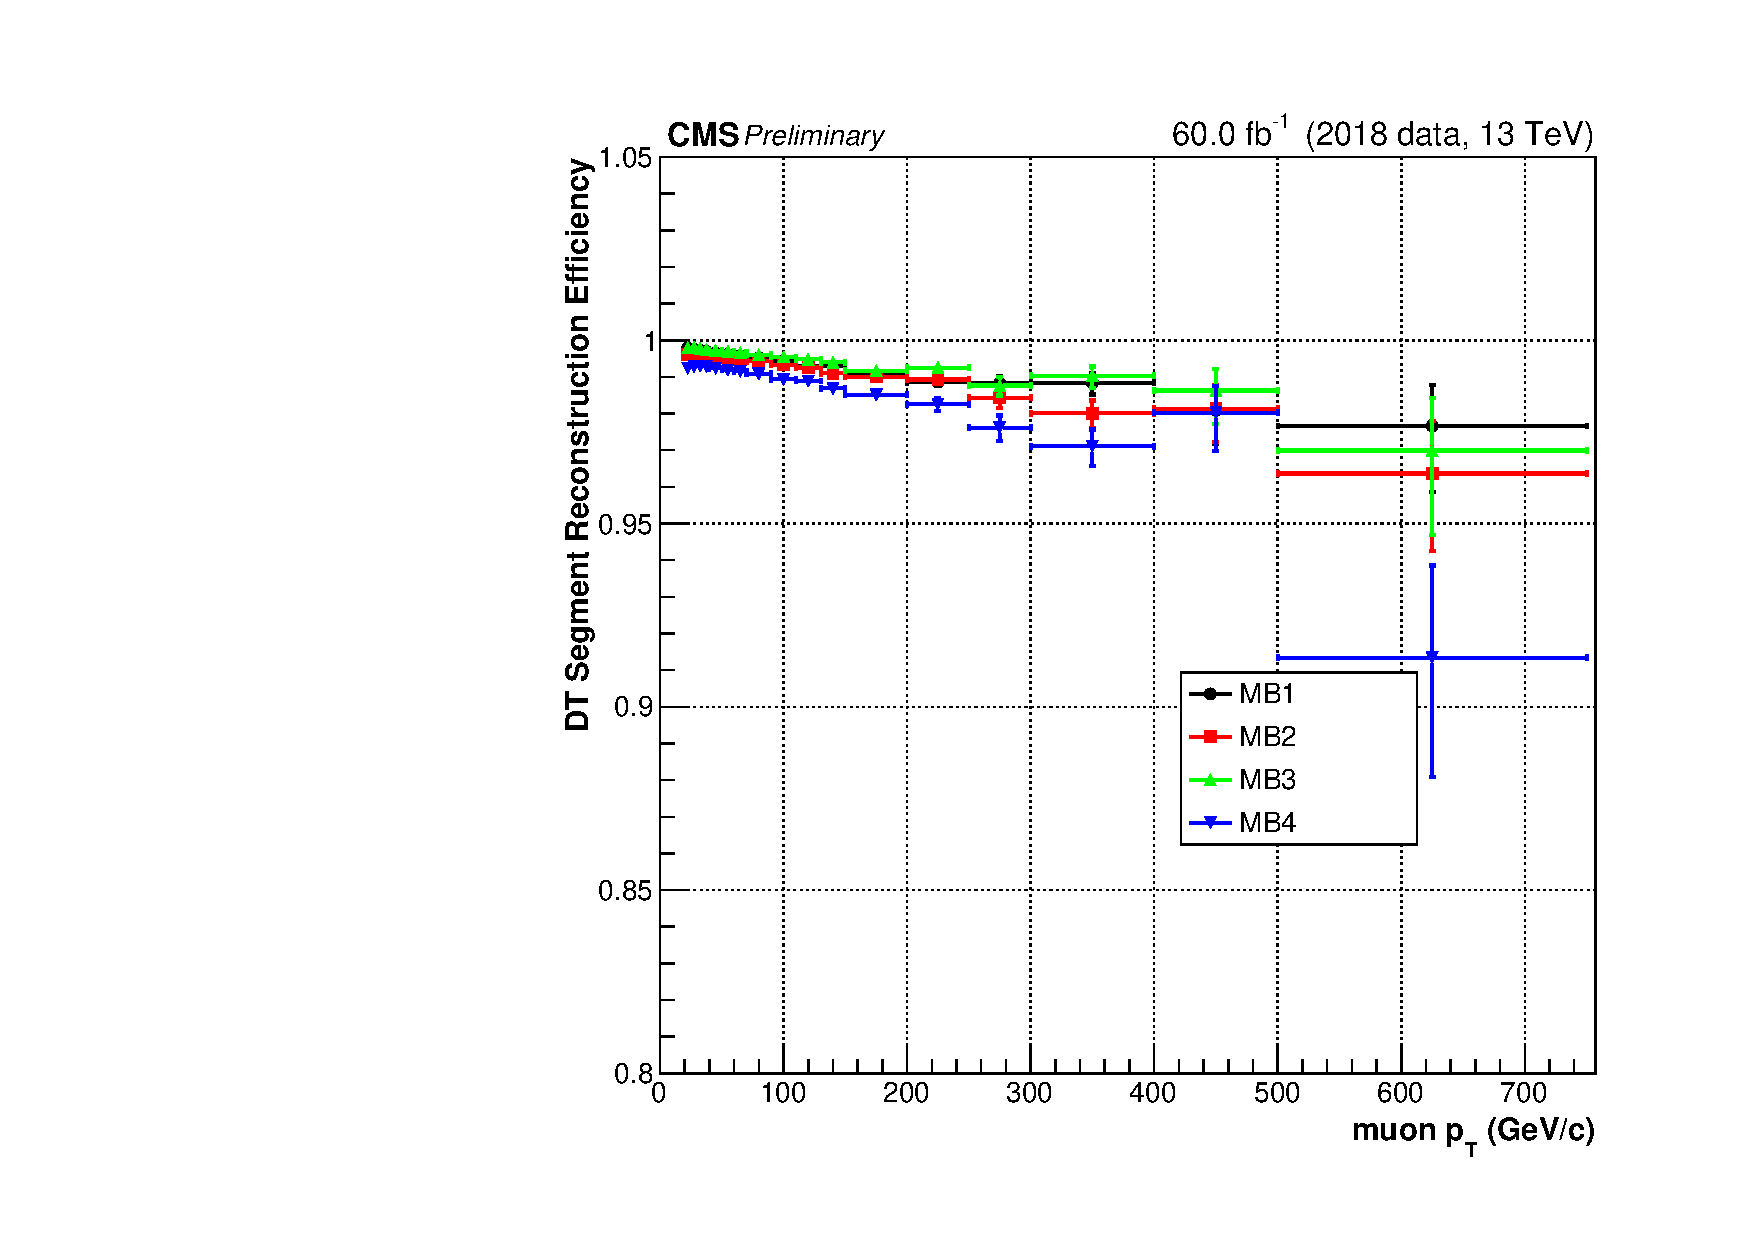
\includegraphics[width=\textwidth]{figures/ShoweringEffect/DT_eff_vs_pt.pdf}}
        \caption{{\scriptsize "The next plot shows the segment efficiency as a function of transverse momentum of the probe muon. It is $\gtrsim$ 99\% up to pT $\le$ 100 GeV and keeps $\approx$ 98\% up to 500 GeV ({\color{uosblue} \textbf{\textit{the mild trend being likely due to showering}}})"}}
        %\label{fig:my_label}
    \end{figure}
\end{column}
\begin{column}{0.5\textwidth}
    \begin{figure}
        \centering
        \href{https://twiki.cern.ch/twiki/bin/view/CMSPublic/MuonDPGPublic160729#CSC_Segment_Efficiency}{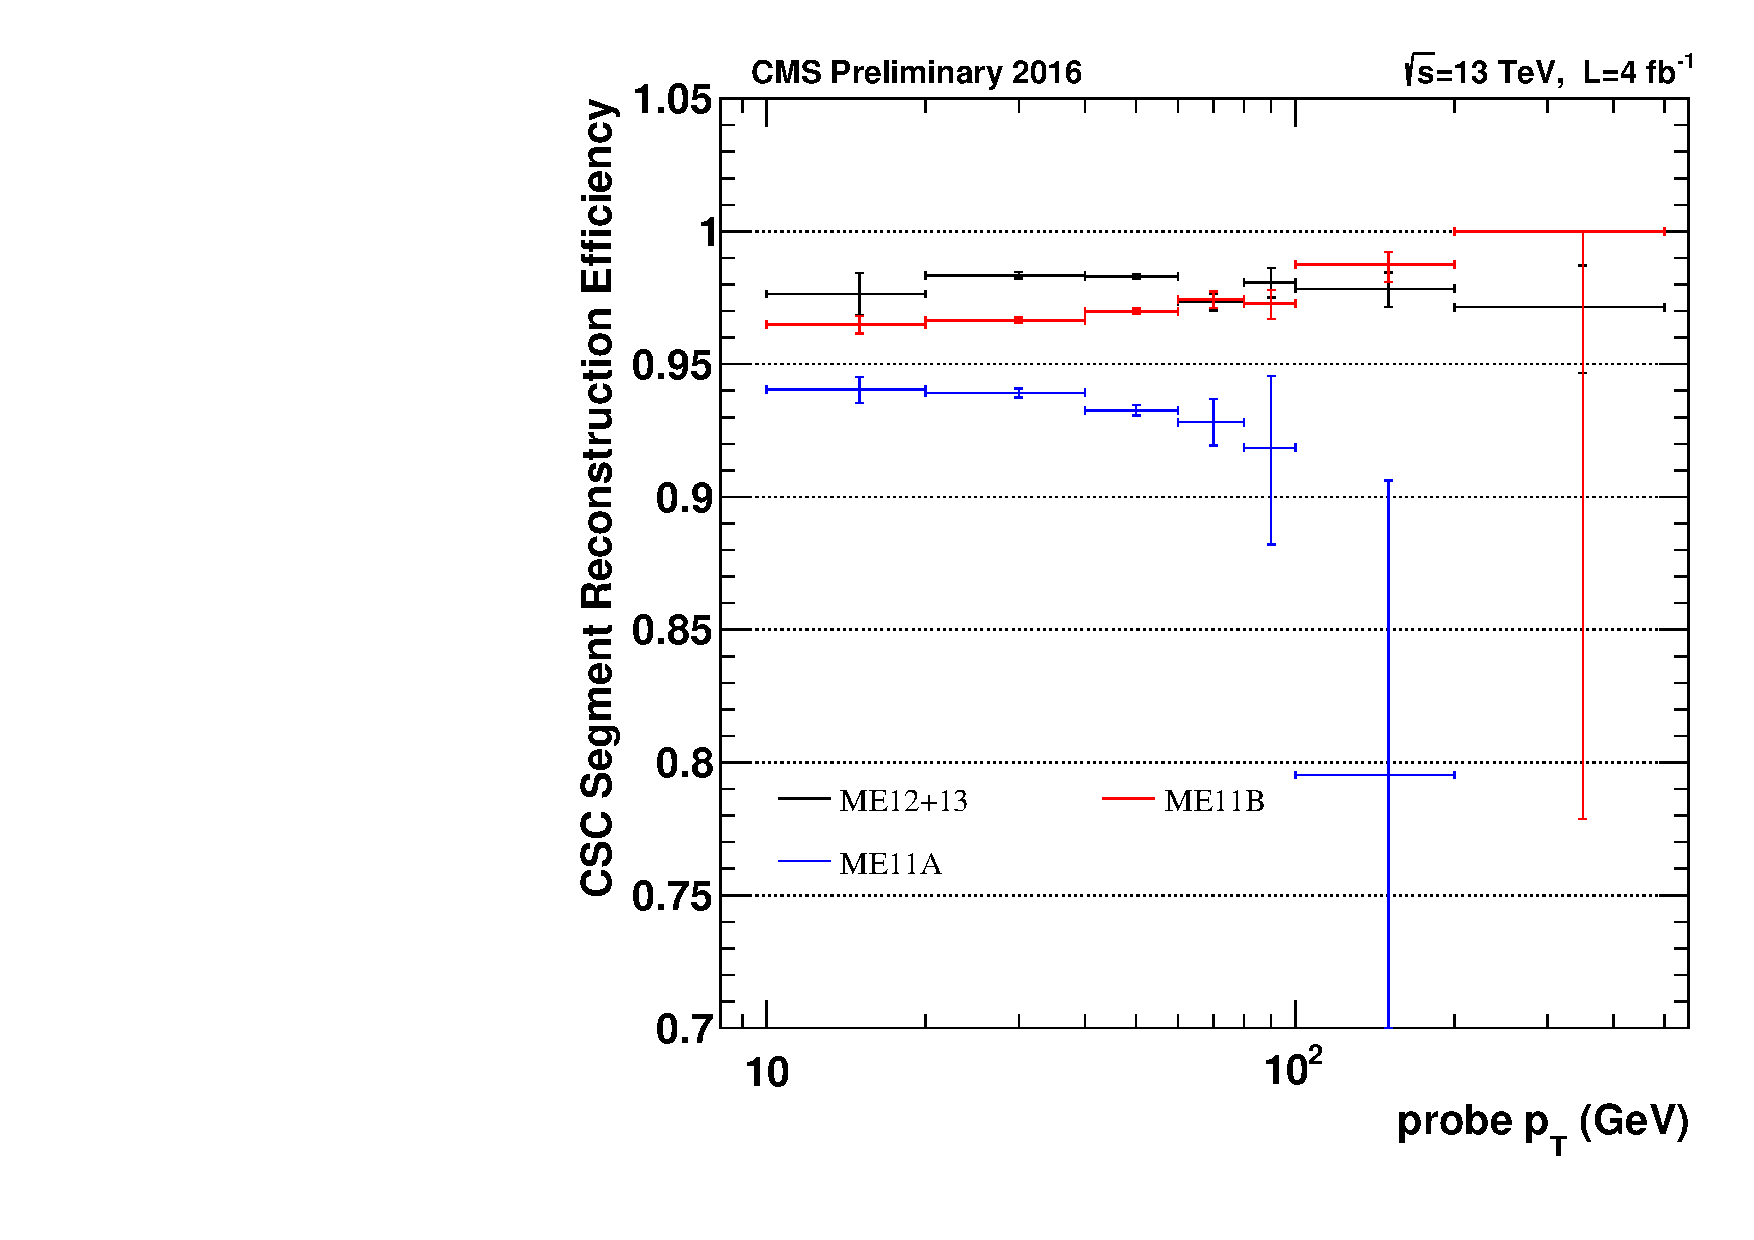
\includegraphics[width=\textwidth]{figures/ShoweringEffect/CSC_seg_eff_JSON_June22all_pt_St_ME1.pdf}}
        \caption{{\scriptsize "Measured efficiency (with statistical uncertainty) of each ring of CSCs in the ME1 station to provide a reconstructed muon track segment, as a function of pT"}}
        %\label{fig:my_label}
    \end{figure}
\end{column}
\end{columns}
\end{frame}


%%%%%%%%%%%%%%%%%%%%%%%%%%%%%%%%%%%%%%%%%%%%%%%%%%%%%%%%%%%%%%%%%%



\begin{frame}[fragile]{Road Usage}

\begin{figure}
    \centering
    \href{https://www.epj-conferences.org/articles/epjconf/pdf/2019/19/epjconf_chep2018_02014.pdf}{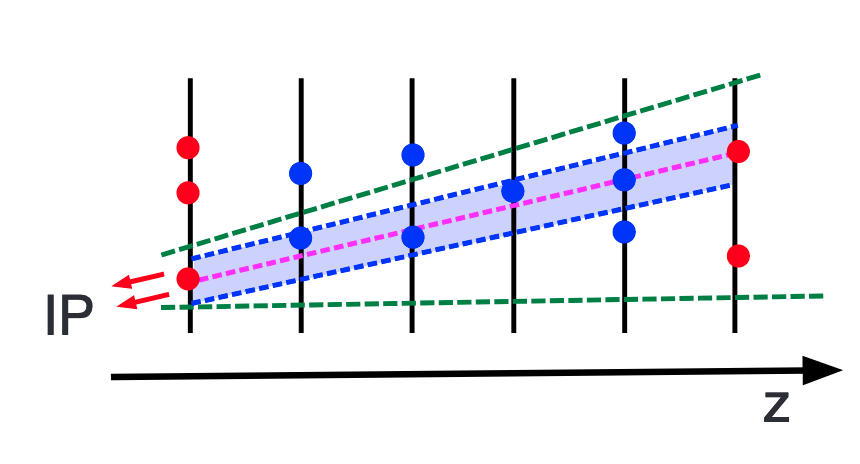
\includegraphics[width=0.32\textwidth]{figures/RU/Schematic-illustration.png}}
    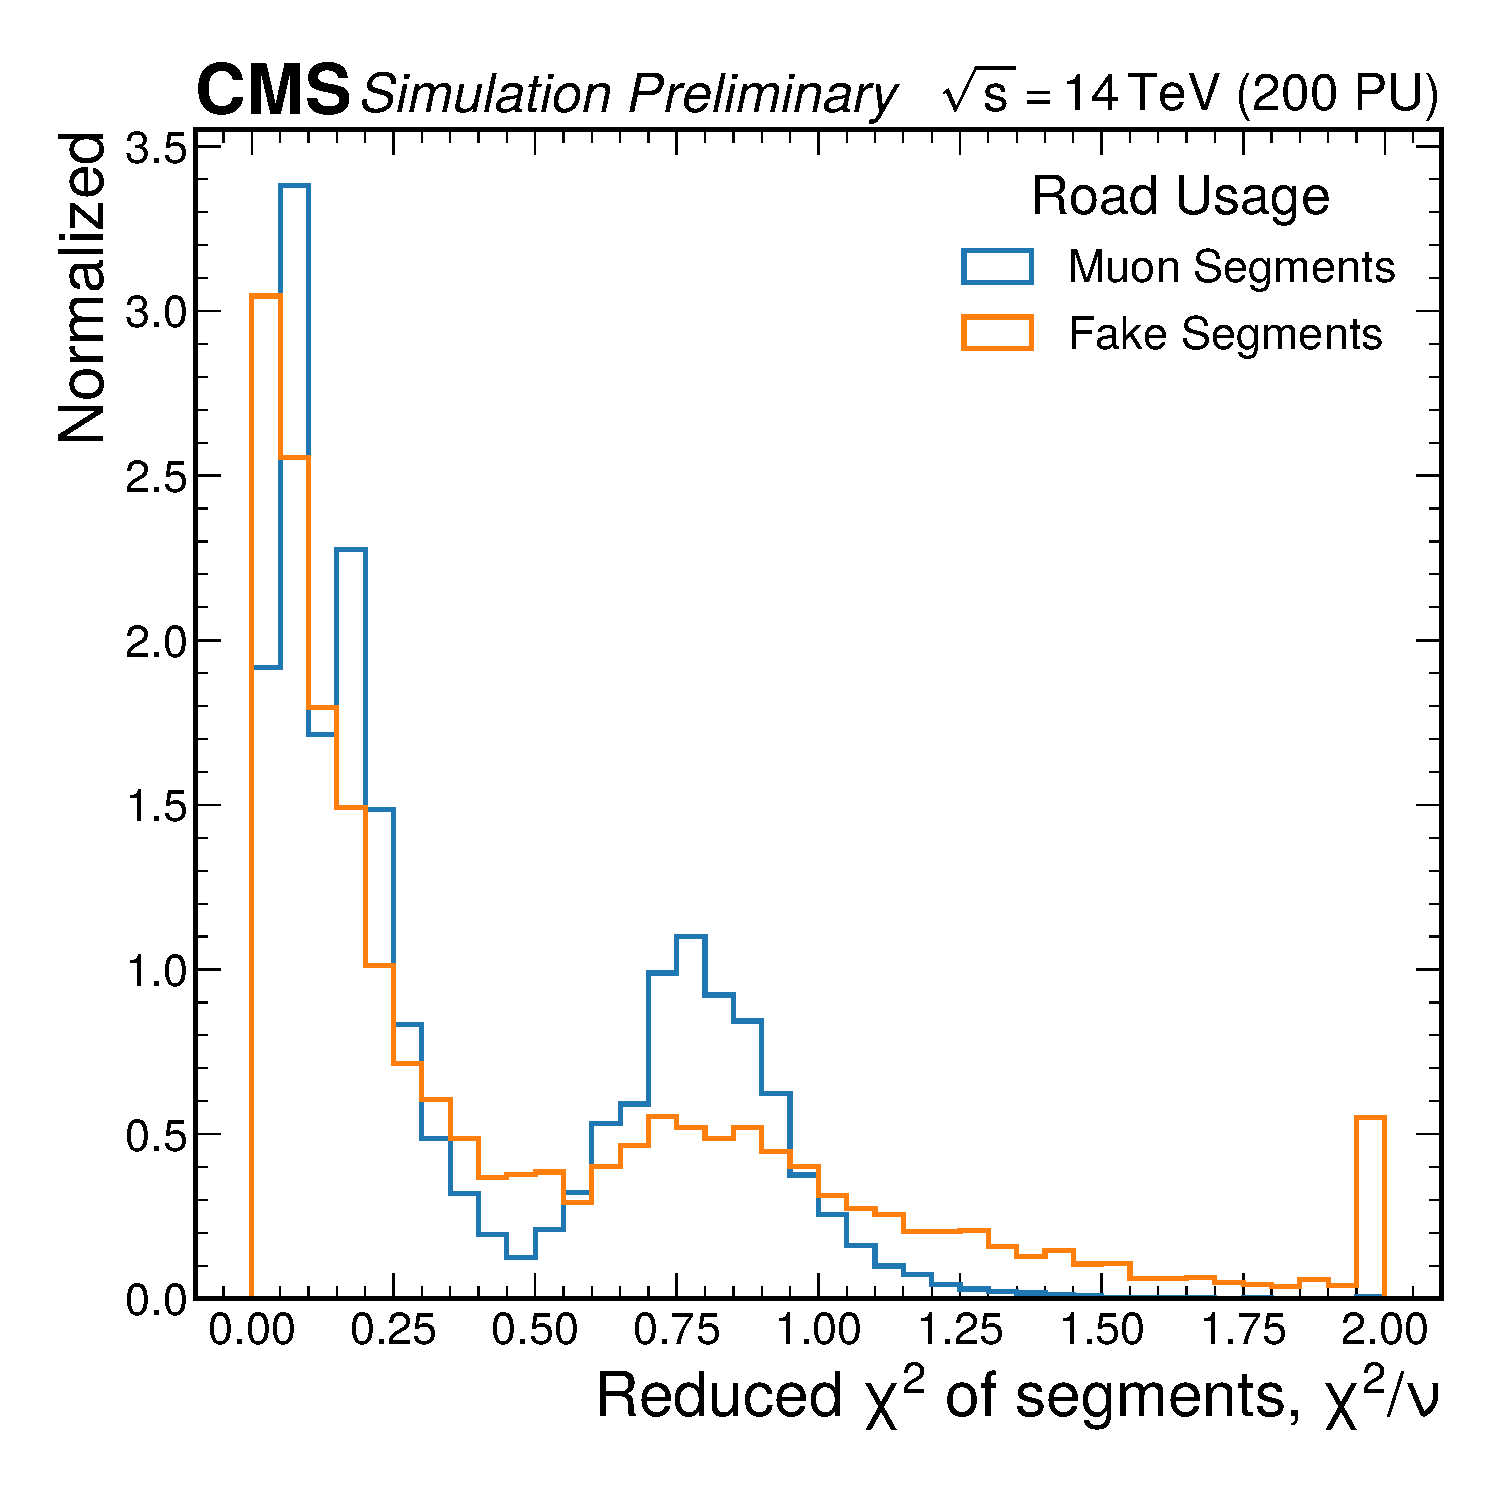
\includegraphics[width=0.32\textwidth]{figures/RU/RU_ReducedChi2.pdf}
    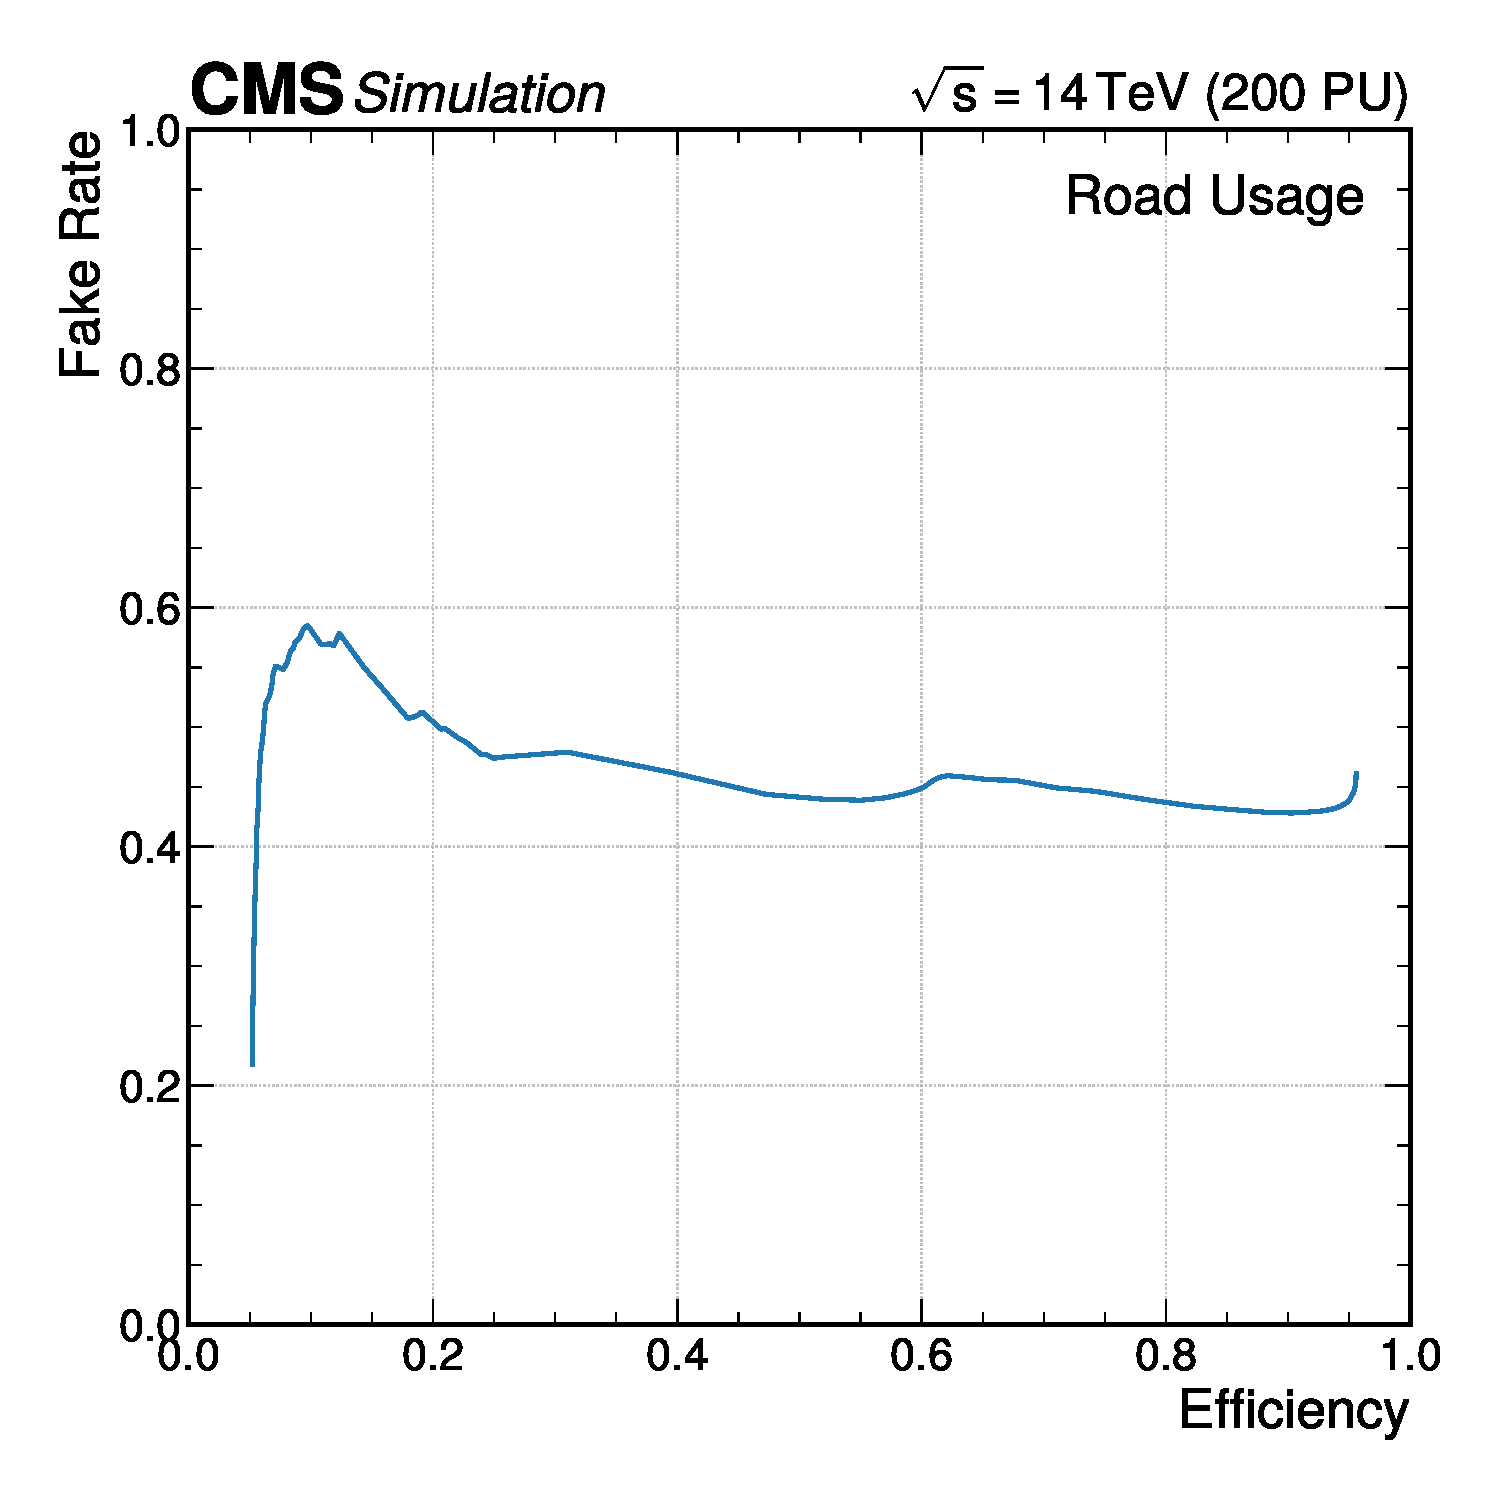
\includegraphics[width=0.32\textwidth]{figures/RU/RU_ROC.pdf}
\end{figure}

\begin{itemize}
    \item Fake rate vs. efficiency curve for Road Usage algorithm was drawn by varying the threshold on the reduced $\chi^{2}$ cut.
    \item The road usage algorithm has a limit in lowering the fake rate alone.
\end{itemize}

\end{frame}


%%%%%%%%%%%%%%%%%%%%%%%%%%%%%%%%%%%%%%%%%%%%%%%%%%%%%%%%%%%%%%%%%%

\begin{frame}[fragile]{Model Visualization (1)}
\begin{columns}
\begin{column}{0.3\textwidth}
\begin{figure}
    \centering
    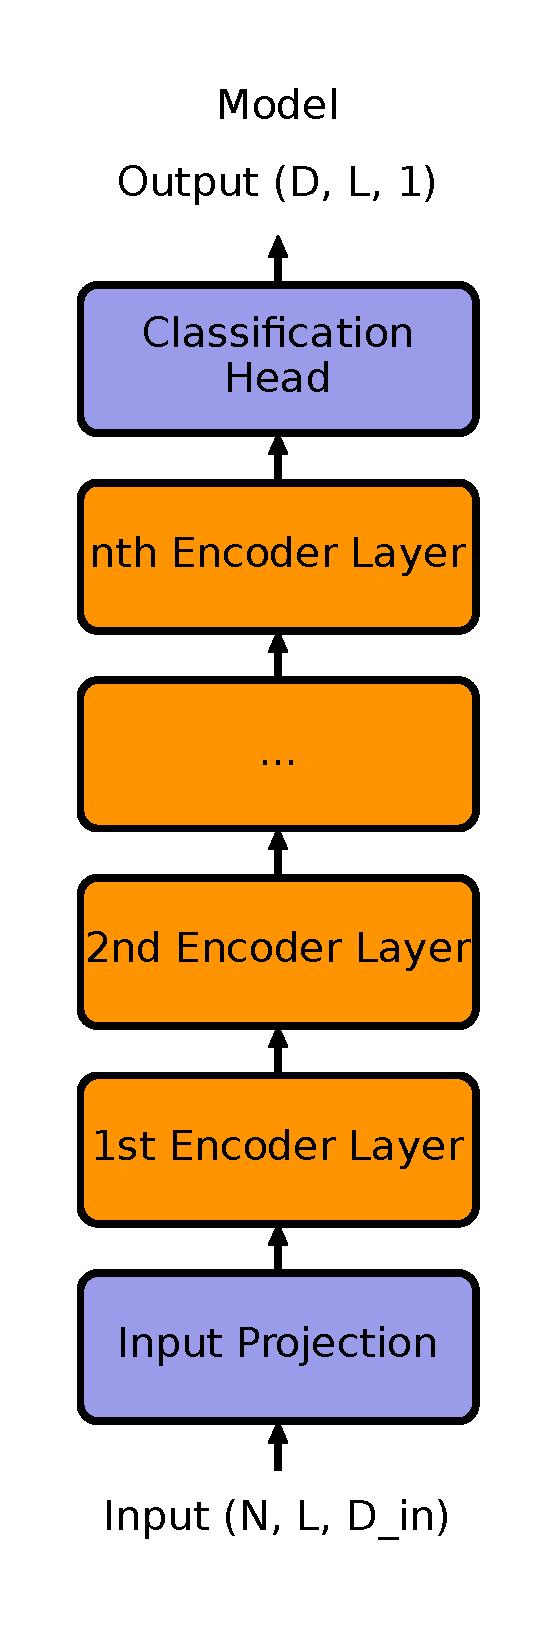
\includegraphics[height=\textheight]{figures/model/model.pdf}
\end{figure}    
\end{column}

\begin{column}{0.3\textwidth}
\begin{figure}
    \centering
    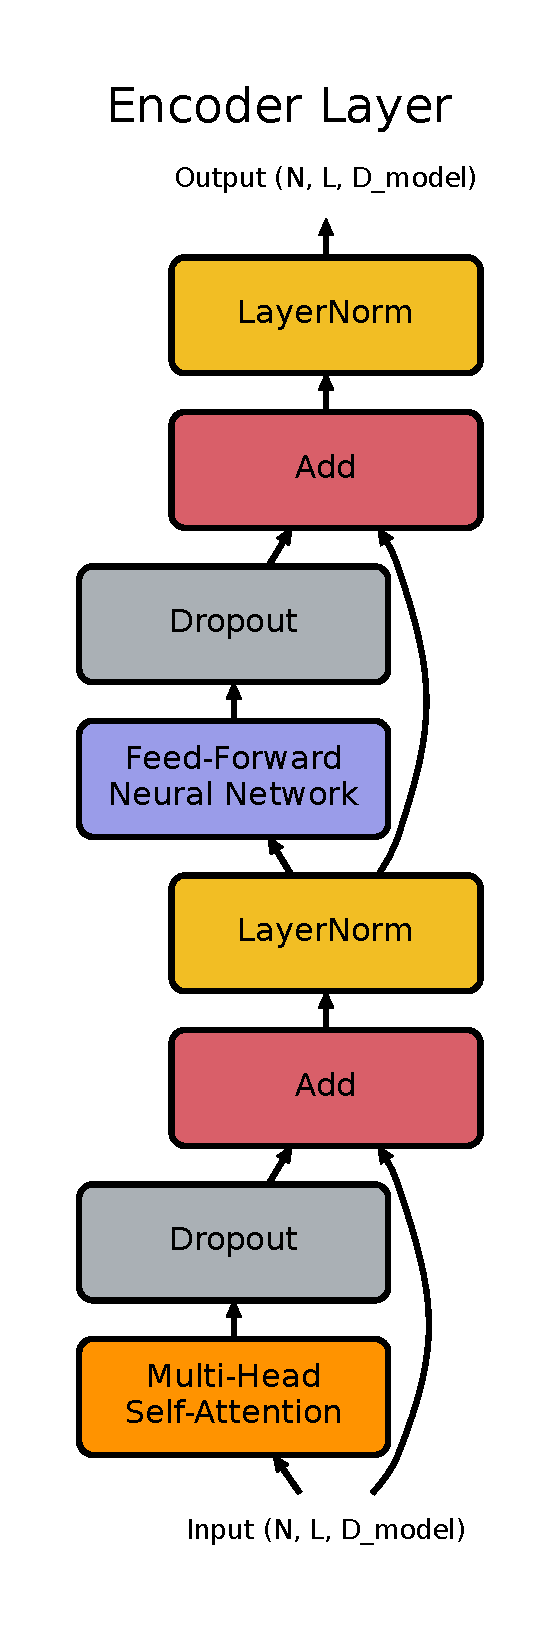
\includegraphics[height=\textheight]{figures/model/encoder-layer.pdf}
\end{figure}    
\end{column}

\begin{column}{0.3\textwidth}
\begin{figure}
    \centering
    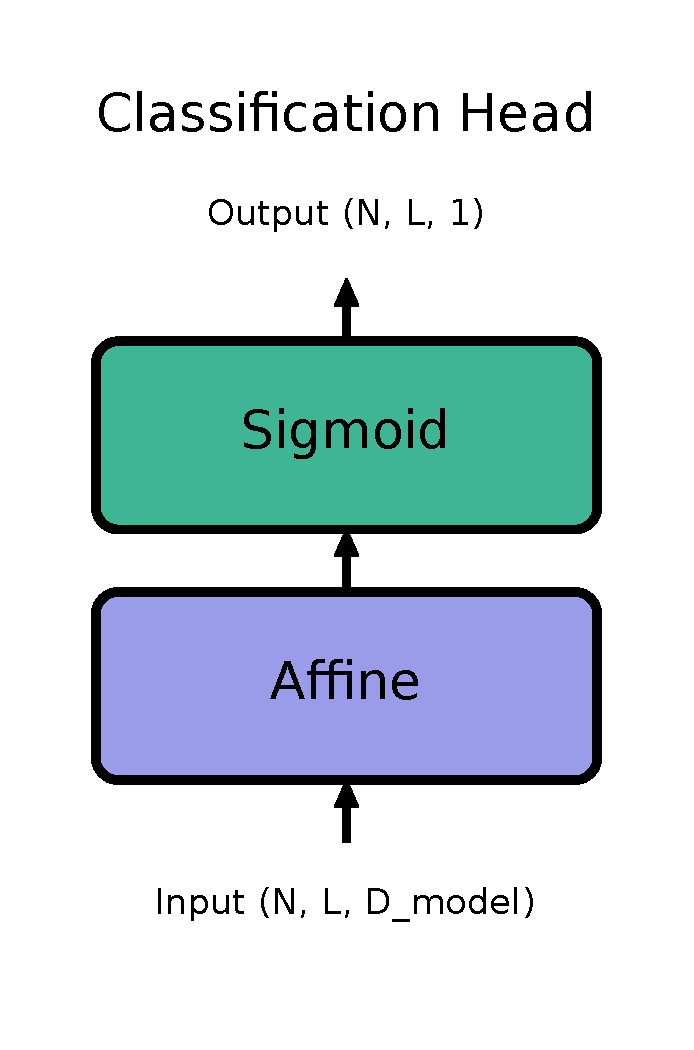
\includegraphics[height=0.4\textheight]{figures/model/simple-output-proj.pdf}
\end{figure}    
\end{column}

\end{columns}

\end{frame}

\begin{frame}[fragile]{Model Visualization (2)}
\begin{columns}
%%%%%%%%%%%%%%%%%%%%%%%%%
\begin{column}{0.3\textwidth}
\begin{figure}
    \centering
    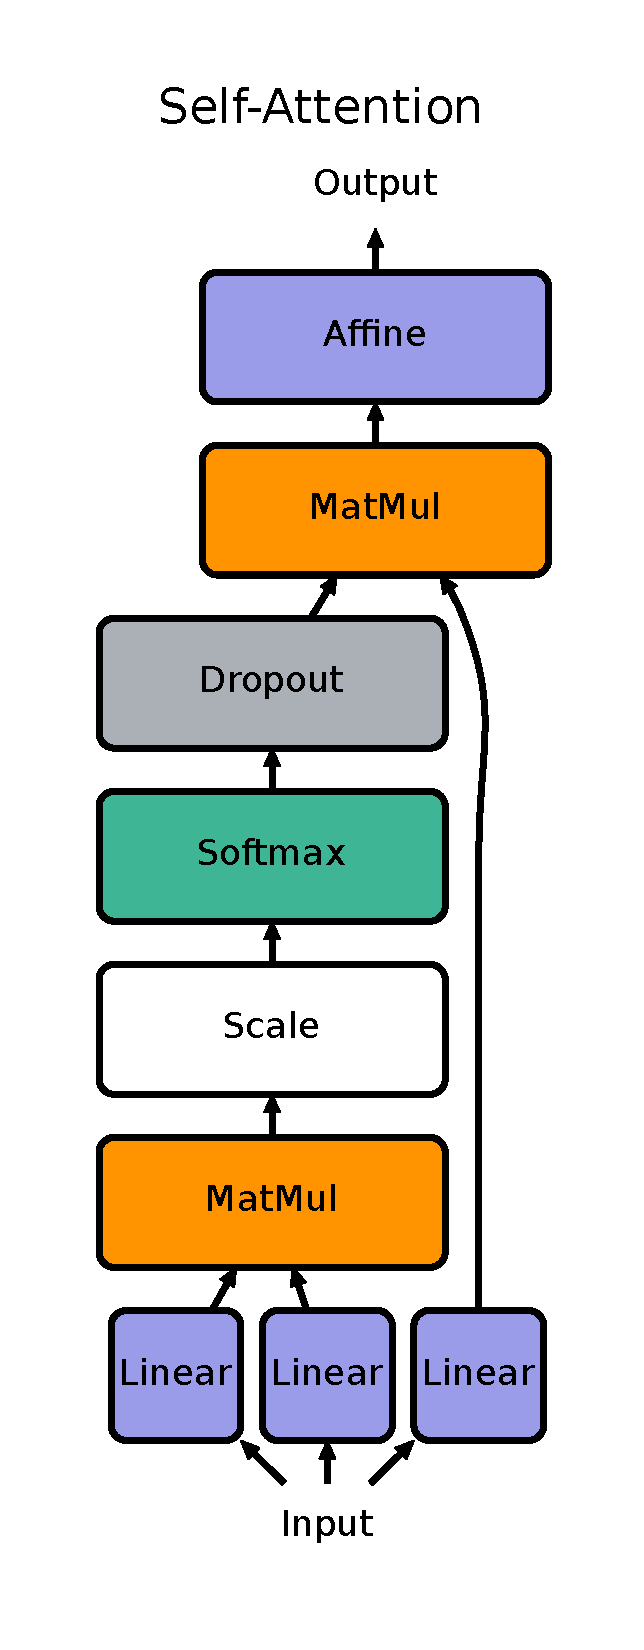
\includegraphics[height=\textheight]{figures/model/self-attention.pdf}
\end{figure}    
\end{column}
%%%%%%%%%%%%%%%%%%%%%%%%%
\begin{column}{0.3\textwidth}
\begin{figure}
    \centering
    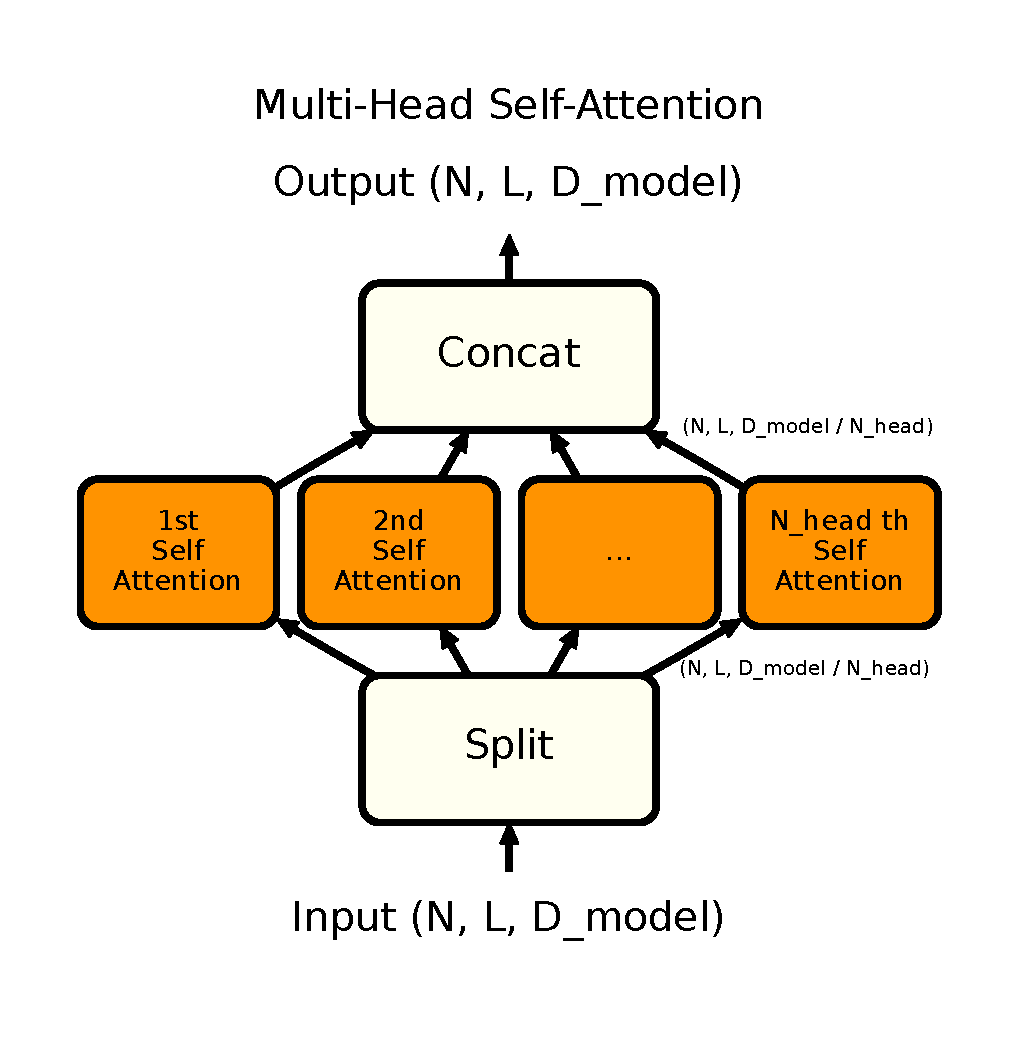
\includegraphics[width=\textwidth]{figures/model/multi-head-self-attention.pdf}
\end{figure}    
\end{column}
%%%%%%%%%%%%%%%%%%%%%%%%%
\begin{column}{0.3\textwidth}
\begin{figure}
    \centering
    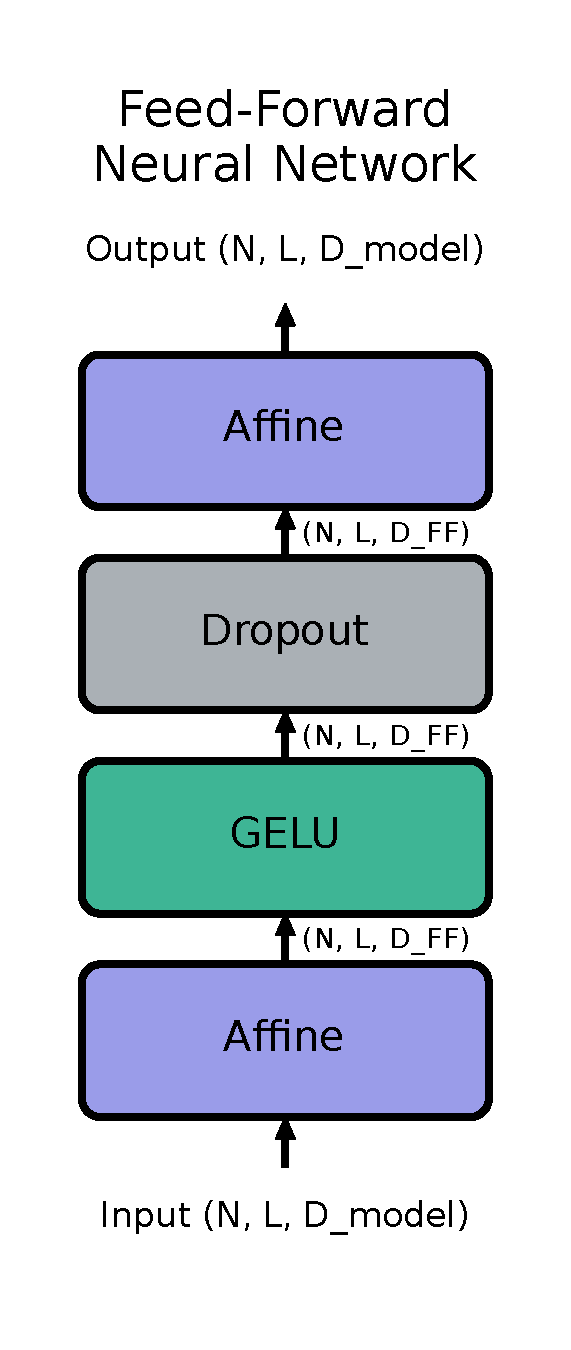
\includegraphics[width=\textwidth]{figures/model/ffnn.pdf}
\end{figure}    
\end{column}
%%%%%%%%%%%%%%%%%%%%%%%%%
\end{columns}
\end{frame}
%%%%%%%%%%%%%%%%%%%%%%%%%%%%%%%%%%%%%%%%%%%%%%%%%%%%%%%%%%%%%%%%%%



\end{document}
